% **************************************************
% Document Class Definition
% **************************************************
\documentclass[%
    paper=A4,               % paper size --> A4 is default in Germany
    twoside=false,           % onesite or twoside printing
    openright,              % doublepage cleaning ends up right side
    parskip=half,           % spacing value / method for paragraphs
    chapterprefix=true,     % prefix for chapter marks
    11pt,                   % font size
    headings=normal,        % size of headings
    bibliography=totoc,     % include bib in toc
    listof=totoc,           % include listof entries in toc
    titlepage=on,           % own page for each title page
    captions=tableabove,    % display table captions above the float env
    appendixprefix=true,    % display a prefix for appendix chapter
    draft=false,            % value for draft version
]{scrreprt}%


% **************************************************
% Setup thesis document
% **************************************************
% !TEX root = thesis.tex


% **************************************************
% Files' Character Encoding
% **************************************************
\usepackage[utf8]{inputenc}


% **************************************************
% Information and Commands for Reuse
% **************************************************
\newcommand{\thesisTitle}{Ohua as an STM alternative for shared state applications}
\newcommand{\thesisName}{Felix Wittwer}
\newcommand{\thesisSubject}{Compiler Construction}
\newcommand{\thesisDate}{May 18, 2020}
\newcommand{\thesisVersion}{Draft-\today}

\newcommand{\thesisFirstReviewer}{Prof. Dr.-Ing. Jeronimo Castrillon}
\newcommand{\thesisFirstReviewerUniversity}{\protect{TU Dresden}}
\newcommand{\thesisFirstReviewerDepartment}{Chair for Compiler Construction}

\newcommand{\thesisSecondReviewer}{Dr.-Ing. Michael Roitzsch}
\newcommand{\thesisSecondReviewerUniversity}{\protect{TU Dresden}}
\newcommand{\thesisSecondReviewerDepartment}{Chair for Operating Systems}

\newcommand{\thesisFirstSupervisor}{Dr.-Ing. Sebastian Ertel}

\newcommand{\thesisUniversity}{\protect{TU Dresden}}
\newcommand{\thesisUniversityDepartment}{Department of Computer Science}
\newcommand{\thesisUniversityInstitute}{Institute of Computer Engineering}
\newcommand{\thesisUniversityGroup}{Chair for Compiler Construction}
\newcommand{\thesisUniversityCity}{Dresden}
\newcommand{\thesisUniversityStreetAddress}{}
\newcommand{\thesisUniversityPostalCode}{01062}


% **************************************************
% Debug LaTeX Information
% **************************************************
%\listfiles


% **************************************************
% Load and Configure Packages
% **************************************************
\usepackage[english]{babel} % babel system, adjust the language of the content
\PassOptionsToPackage{% setup clean thesis style
    figuresep=colon,%
    hangfigurecaption=false,%
    hangsection=true,%
    hangsubsection=true,%
    sansserif=false,%
    configurelistings=true,% -- ?
    colorize=full,%
    colortheme=bluemagenta,%
    configurebiblatex=true,%
    bibsys=biber,%
    bibfile=bib-refs,%
    bibstyle=numeric,%
    bibsorting=nty,% -- ?
}{cleanthesis}
\usepackage{cleanthesis}

\hypersetup{% setup the hyperref-package options
    pdftitle={\thesisTitle},    %   - title (PDF meta)
    pdfsubject={\thesisSubject},%   - subject (PDF meta)
    pdfauthor={\thesisName},    %   - author (PDF meta)
    plainpages=false,           %   -
    colorlinks=false,           %   - colorize links?
    pdfborder={0 0 0},          %   -
    breaklinks=true,            %   - allow line break inside links
    bookmarksnumbered=true,     %
    bookmarksopen=true          %
}

% **************************************************
% Other Packages
% **************************************************
\usepackage{scrhack}
\usepackage[textsize=tiny]{todonotes}
\usepackage{graphicx}
\usepackage{subcaption}

% minted
\usepackage[chapter]{minted}
\setminted{autogobble=true, linenos=true, breaklines=true}
\usemintedstyle{friendly}

\renewcommand{\listoflistingscaption}{\textbf{List of Listings}}



% **************************************************
% Own commands for use within the thesis
% **************************************************

\newcommand{\rust}[1]{\mintinline{rust}{#1}}


\renewcommand{\baselinestretch}{1.0}


% **************************************************
% Document CONTENT
% **************************************************
\begin{document}

% uncomment the following command to fill up pages with
% whitespace instead of aligning the first and last lines
% of a page (see \raggedbottom vs. \flushbottom)
%\raggedbottom

% --------------------------
% rename document parts
% --------------------------

% > set short label names for floating environments figure and table
%\renewcaptionname{ngerman}{\figurename}{Abb.}
%\renewcaptionname{ngerman}{\tablename}{Tab.}
\renewcaptionname{english}{\figurename}{Fig.}
\renewcaptionname{english}{\tablename}{Tab.}

% > rename the title of the LOL, i.e. list of listings (default is "Listings")
% \renewcommand*{\lstlistlistingname}{List of Listings}

% --------------------------
% Front matter
% --------------------------
\pagenumbering{roman}			% roman page numbing (invisible for empty page style)
\pagestyle{empty}				% no header or footers
% !TEX root = ../thesis.tex
%
% ------------------------------------  --> cover title page
\begin{titlepage}
	\pdfbookmark[0]{Cover}{Cover}
	\flushright
	\hfill
	\vfill
	{\LARGE \textsc{Master's Thesis}}
	
	{\LARGE\thesisTitle \par}
	\rule[5pt]{\textwidth}{.4pt} \par
	{\Large\thesisName}
	\vfill
	\textit{\large\thesisDate} \\
	Version: \thesisVersion
\end{titlepage}


% ------------------------------------  --> main title page
\begin{titlepage}
	\pdfbookmark[0]{Titlepage}{Titlepage}
	\tgherosfont
	\centering

    % 
\includegraphics[height=0.06\textheight]{gfx/tudlogo}
	% \hfill
    % 
\includegraphics[height=0.06\textheight]{gfx/cc-logo}
    % or ...
	% {\Large \thesisUniversity} \\[4mm]
	
\includegraphics[width=6cm]{gfx/tudlogo} \\[2mm]
	\textsf{\thesisUniversityDepartment} \\
	\textsf{\thesisUniversityInstitute} \\
	\textsf{\thesisUniversityGroup} \\

	\vfill
	{\Large \textsc{Master's Thesis}} \\[5mm]
	{\LARGE \color{ctcolortitle}\textbf{\thesisTitle} \\[10mm]}
	{\Large \thesisName} \\

	\vfill
	\begin{minipage}[t]{.27\textwidth}
		\raggedleft
		\textit{1. Reviewer}
	\end{minipage}
	\hspace*{15pt}
	\begin{minipage}[t]{.65\textwidth}
		{\Large \thesisFirstReviewer} \\
	  	{\small \thesisFirstReviewerDepartment} \\[-1mm]
		{\small \thesisFirstReviewerUniversity}
	\end{minipage} \\[5mm]
	\begin{minipage}[t]{.27\textwidth}
		\raggedleft
		\textit{2. Reviewer}
	\end{minipage}
	\hspace*{15pt}
	\begin{minipage}[t]{.65\textwidth}
		{\Large \thesisSecondReviewer} \\
	  	{\small \thesisSecondReviewerDepartment} \\[-1mm]
		{\small \thesisSecondReviewerUniversity}
	\end{minipage} \\[10mm]
	\begin{minipage}[t]{.27\textwidth}
		\raggedleft
		\textit{Supervisor}
	\end{minipage}
	\hspace*{15pt}
	\begin{minipage}[t]{.65\textwidth}
		\thesisFirstSupervisor
	\end{minipage} \\[10mm]

	\thesisDate \\

\end{titlepage}


% ------------------------------------  --> lower title back for single page layout
\hfill
\vfill
{
	\small
	\textbf{\thesisName} \\
	\textit{\thesisTitle} \\
	\thesisSubject, \thesisDate \\
	Reviewers: \thesisFirstReviewer\ and \thesisSecondReviewer \\
	Supervisor: \thesisFirstSupervisor \\[1.5em]
	\textbf{\thesisUniversity} \\
	\textit{\thesisUniversityGroup} \\
	\thesisUniversityInstitute \\
	\thesisUniversityDepartment \\
	% \thesisUniversityStreetAddress \\
	\thesisUniversityPostalCode\ \thesisUniversityCity
}
		% INCLUDE: all titlepages
\cleardoublepage

% TODO: Add task description somewhere!

% TODO: Add abstract
% \pagestyle{plain}				% display just page numbers
% % !TEX root = ../thesis.tex
%
\chapter*{Abstract}
\label{sec:abstract}

The efficient parallelization of shared state applications has been an ongoing research topic ever since the advent of multi-core processors.
Due to the properties some of these programs exhibit, such as amorphous data parallelism and the use of pointer-based data structures, conventional concurrency control mechanisms like locking fail to uncover any meaningful parallelism.
Speculative parallelism approaches have been developed as a result, the most prominent representative being \emph{Software Transactional Memory}.
But these frameworks have their own set of drawbacks like the lack of scalability and high overheads.
It is unclear, whether approaches like implicit parallelism could be a feasible and more performant alternative to use for developing these applications.

This thesis tries to find out, whether \emph{Ohua}, a framework for exploiting implicit parallelism, could be used for writing shared state programs and whether it could be an alternative to the by now aged STM.
In order to do this, we tested in a preliminary study Ohua's usability in shared state environments. % as this had not been tested yet.
We then proposed a set of transformations for Ohua to run at compile-time to automatically recognize and exploit parallelism from such applications.
To compare Ohua then against STM, we tested both in a series of benchmarks that ressemble real-world applications.

The evaluation shows that Ohua is not able to exploit parallelism in shared state applications to the same degree as STM does.
Nonetheless, Ohua shows results that are widely on par with Software Transactional Memory and performs especially good in applications with amorphous data parallelism, validating our proposed transformations.
		% INCLUDE: the abstracts (english and german)
% \cleardoublepage
% - keep this comment here!
% TODO: Add acknowledgements
% \input{chapters/acknowledgement} % INCLUDE: acknowledgement
% \cleardoublepage
% - keep this comment here!
\currentpdfbookmark{\contentsname}{toc}
\setcounter{tocdepth}{2}		% define depth of toc
\tableofcontents				% display table of contents
\cleardoublepage

% --------------------------
% Body matter
% --------------------------
\pagenumbering{arabic}			% arabic page numbering
\setcounter{page}{1}			% set page counter
\pagestyle{maincontentstyle}			% header and footer style
% \pagestyle{scrheadings}			% header and footer style

%% Uncomment the following lines using the \part command
%% to add part sections
%\part{Example Part}
% !TEX root = ../thesis.tex
%
\chapter{Introduction}
\label{sec:introduction}

At the beginning of the century, it became apparent that advancements in CPU architecture were hitting the power wall.
Clock speeds of single cores could no longer be increased without also increasing the power dissipation of the unit beyond the capabilities of consumer-grade cooling solutions.
Multi-core architectures and technologies like Intel's hyperthreading soon emerged as possible solutions to this problem, making exploiting parallelism a viable option to improve performance.
Since most programs modify state in some way, primitives that allow the safe sharing of such state became an important tool.

\emph{Software Transactional Memory}~\cite{shavit1997software} is a framework that allows state sharing without exposing low-level mechanisms like locks to the developer, the use of which usually severely degrades the reliability of the resulting code.
Instead, the framework allows the definition of so-called atomic blocks, code sections in which all changes made to shared data are either written successfully or not at all, similar to database transactions.
This framework has now been an integral tool for state sharing for a while, yet it has a number of problems that have been widely reported in research, such as a lack of scalability~\cite{perfumo2008limits} and too high framework overheads~\cite{cascaval2008software}.
When we inspected and used STM code written as part of the widely used STAMP benchmark suite~\cite{minh2008stamp}, we also encountered issues:\todo{noch mal bisschen Formulierungsarbeit investieren hier}
Even the code provided for some benchmarks does not always produce a correct result for the computation it implements, serving as example for how hard it is to correctly write a program using Software Transactional Memory.
Worse, using STM actually makes memory management inside the application even harder, as several irregularly occurring memory management issues prove.
Finally, even though Software Transactional Memory aimed to relief the programmer of the burden to manage locks manually, the framework itself may introduce deadlocks into the application, as we will see.
Although this may be traced back to a bug within the framework itself this shows impressively that the implementation of this framework is indeed not trivial and that proving the correctness of the framework is hard.

\emph{Ohua}~\cite{ertel2015ohua}, on the other hand, does not have these problems.
Proposed by Ertel et al., the frameworks allows the creation of implicitly parallel programs.
Using a number of transformations, parallelism is extracted from an otherwise sequential piece of code.
The resulting dataflow graph is then translated into a runtime which exploits the found parallelism.
Both of these steps can be checked for correctness relatively easily, leaving only the sequential code correctness to the developer.
Its underlying deterministic model additionally ensures that sporadically arising bugs as observed in the STAMP suite cannot occur.
Unfortunately, Ohua achieves most of its guarantees because it only fosters local state to avoid the need for locking.
Thus, it is incapable of handling shared state as of now.

In this thesis, we want to test the usability of Ohua in shared state applications.
Therefore, we will look at the theoretical foundations of the framework to see, whether they allow an extension to shared state.
In order to then properly evaluate Ohua in this context, we are going to compare its performance to that of STM, a well-established shared state programming framework, to see whether it could indeed be a suitable alternative to use for writing these applications.
We make the following contributions:\todo{Überarbeiten bzw ausbauen!}

\begin{itemize}
    \item Preliminary studies regarding the feasibility of applying Ohua to shared state scenarios where we tested, whether its theoretical foundations allow the introduction of parallelism in such applications.
    \item Descriptions and definitions of transformations for the Ohua compiler to run on input algorithms to enable it to automatically extract parallelism from shared state applications.
    \item A set of experiments where we applied Ohua to a number of such applications to test its performance in comparison to the STM framework.
    % \item Updated benchmark results for
\end{itemize}

The rest of this thesis is structured as follows:
At first, we will introduce some basic notions and concepts necessary to understand this thesis as well as the motivation for possibly replacing STM in Chapter~\ref{sec:background}.
Then, we will present our preliminary studies about whether or not Ohua's theoretical foundations allow shared state handling in Chapter~\ref{sec:preliminary}.
The resulting amendments that have to be made to the Ohua compiler will be defined in chapter~\ref{sec:transformations} and applied manually to a set of benchmarks in Chapter~\ref{sec:experiments}.
Chapter~\ref{sec:evaluation} will then evaluate and interpret the results of the benchmarks.
Related work on other possible STM replacements is presented in Chapter~\ref{sec:related}.
The thesis will then close with future work presented in Chapter~\ref{sec:future} before concluding in Chapter~\ref{sec:conclusion}.

% !TEX root = ../thesis.tex
%
\chapter{Background and Motivation}%
\label{sec:background}

In this chapter, we are going to introduce the parallelism frameworks \emph{Software Transactional Memory} and \emph{Ohua} as a foundation for the following chapters.
To better understand how one can make a well-founded comparison between both concepts, we will also introduce the class of \emph{Irregular Applications} as well as the term \emph{Amorphous Data Parallelism}.
We will also briefly discuss the difficulties that arise when reasoning about said application types and motivate, why further research into this topic could prove valuable.

\section{Software Transactional Memory}
\label{sec:background:stm}

With the invention of multi-threaded programming, a need for synchronization primitives arose to allow safe parallelization of data-processing applications.
Usually, locks have been used by developers to guard access to pieces of shared data.

Lock-based programming however, has the fundamental drawback of easily producing deadlocks (i.e., a state where a number of threads may never again progress) when acquiring locks in the wrong order, forcing developers to employ great care when using them.
This results in a lack of composability, as combining several small lock-based modules into a larger program would require the imposition of some sort of ordering on the locks, which frequently leads to problems.
Even when written correctly, lock-based programs tend to quickly become hard to read and maintain due to the many rules that need to be enforced by the programmer herself without any external checks.
Another problem is lock contention.
If a lock is currently taken, all other threads seeking to acquire it have to wait.
This opens up a new set of problems as frequent waiting leads to prolonged execution times and waiting threads can starve, should the thread fail to release the lock for any reason.
Mitigating contention issues forces developers to consider the trade-off between the overhead introduced by many fine-grained locks, the resulting higher chance of an accidental deadlock and high contention.

\begin{figure}[h]
    \begin{subfigure}[h]{\textwidth}
    \begin{minted}{Rust}
        let data = TVar::new(12);   // data is a transaction variable
        thread::spawn(move || {
            atomically(|trans| {    // closure for transaction blocks
                let local = data.read(trans)?;
                data.write(trans, local + 2)
            })});
        thread::spawn(move || {
            atomically(|trans| {
                let local = data.read(trans)?;
                data.write(trans, local * 2)
            })});
    \end{minted}
    \caption{Rust code for both transactions.}%
    \label{fig:background:stmcode}
    \end{subfigure}
    \begin{subfigure}[h]{\textwidth}
    \centering
    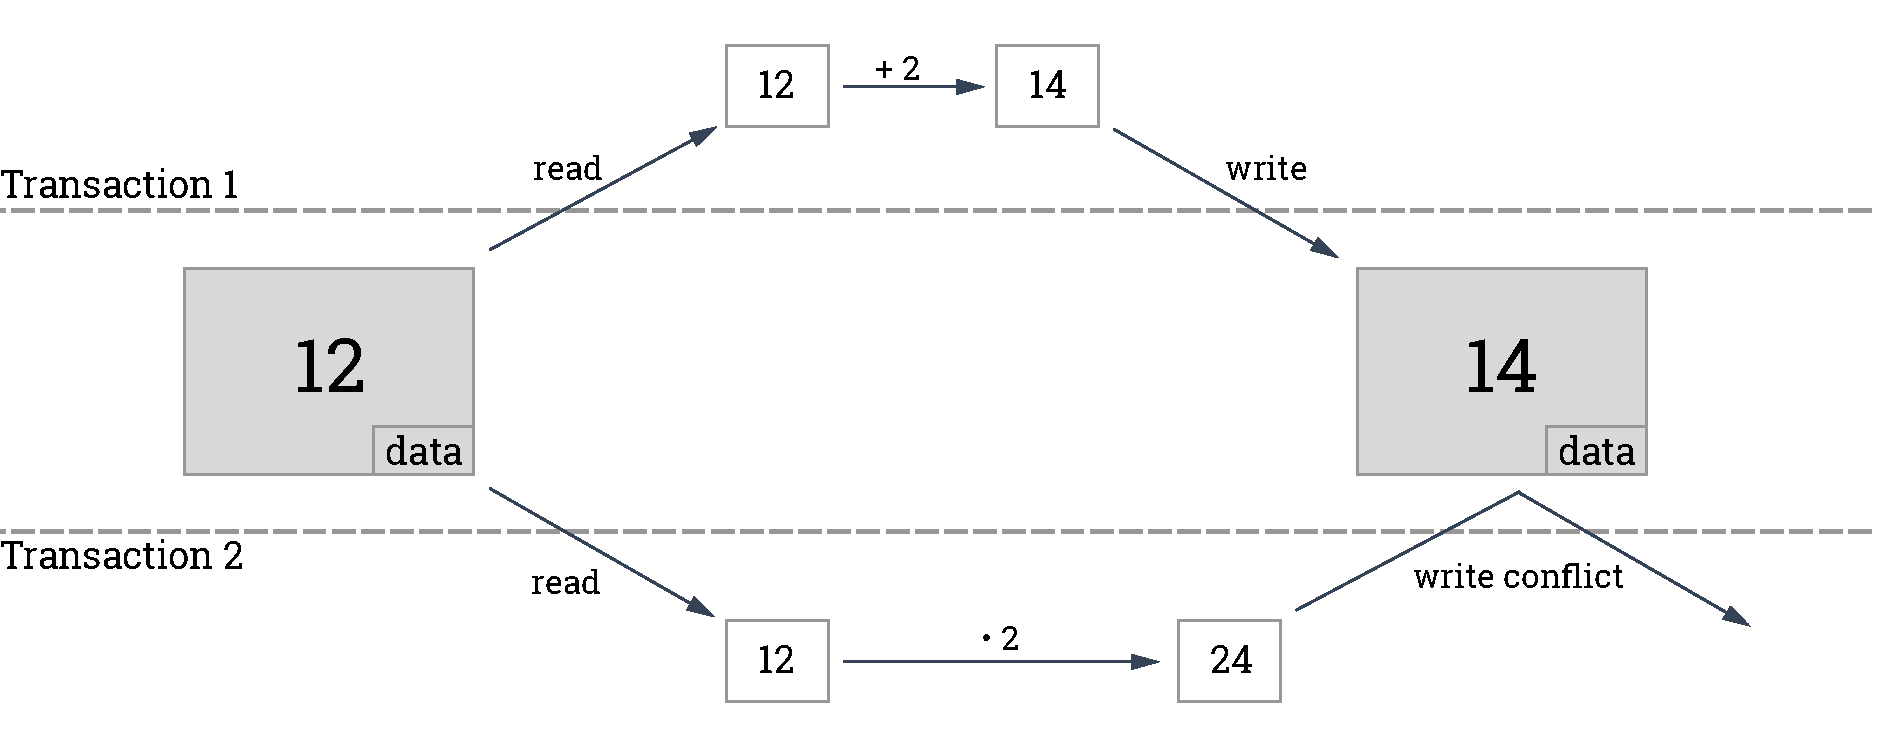
\includegraphics[width=.9\textwidth,keepaspectratio]{gfx/background-stm}
    \caption{Sample execution of two parallel transactions where one transaction has to be rolled back due to a write conflict.}%
    \label{fig:background:stmflow}
    \end{subfigure}
    \caption{Example of two transactions modifying the same shared value in different transactions.}%
    \label{fig:background:stm}
\end{figure}

Hence, Shavit et al.~\cite{shavit1997software} proposed a concept called \emph{Software Transactional Memory}.
This new approach to synchronization aimed to provide lock-free parallelism abstractions that allow multiple threads access to a shared variable without any form of blocking.
Former critical sections are now regarded as \emph{transactions}: They are either executed in their entirety with all their changes taking effect simultaneously or are not executed at all, just like transactions in databases.
STM's operating principle is outlined in Figure~\ref{fig:background:stm} along with a code example in Fig.~\ref{fig:background:stmcode}.
Every read and write operation to or from a piece of shared data is conducted inside a transaction block and gets initially saved to a local transaction log.
When the transaction block comes to an end, the changes made to individual shared data sections are committed.
Therefore, the changes in the log are applied to the original shared values.
In case another transaction managed to commit in the meantime to a value our transaction also touched, the conflict is detected and instead of committing the changes the transaction is aborted and restarted.
This is normally done until the transaction committed successfully.

In our example in Fig.~\ref{fig:background:stm}, the transactions 1 and 2 both read the same value and modify it.
But since the first transaction was able to commit earlier, the second transaction now stands in conflict and has to be aborted and scheduled for re-execution.

As the example already shows, a fundamental benefit of the (Software) Transactional Memory model is its serializability~\cite{swalens2016transactional}:
All transactions seem to execute serially, since the steps of one transaction never appear to be interleaved with the steps of another transaction.
Therefore, the results of an execution must be equal to the result of a serial execution.
This has been formalized by Swalens et al.~\cite{swalens2016transactional} in their proposed operational semantics for a language with transactions.

Overall, STM takes an optimistic approach to parallelism, because it simply executes numerous computations without any heuristics or reasoning in parallel, hoping for as few conflicts as possible.
The result of this is an underlying non-determinism that ensues everytime transactions are employed in a multi-threaded environment.
Problems in this strategy become apparent when applied to high-contention scenarios.
Since STM may work in parallel over the same data structure or memory region, high contention always leads to a significantly increased number of retries for individual executions, which in turn leads to drastically reduced performance.
Further shortcomings of this concept have been discussed in detail by Caşcaval et al.~\cite{cascaval2008software}.
One the one hand, exception handling becomes impossible to do inside of a transaction without breaking its semantics.
On the other hand, I/O operations cannot be transactionalized, as well as anything else that produces side effects outside of the transactions' scope as these effects may not be rolled back on error.
Additionally, they reported large overheads of STM applications for smaller worksets as well as no debuggability, since the non-determinism makes a specific situation nearly irreproducable.


\section{Ohua}
\label{sec:background:ohua}

As we have seen before, most frameworks for parallel programming offer developers certain abstractions or data structures such as threads, locks or transactions for them to use when developing parallel programs.
This however, forces programmers to think within the boundaries of their chosen tools and produces code that is tailored to a specific framework and therefore hard to migrate.

A completely different approach has been taken by Ertel et al.~\cite{ertel2019dis} with the proposition of \emph{Ohua}, which is a framework that allows the development of implicitly parallel programs.
It consists of three main components, as outlined in Fig.~\ref{fig:background:ohua}:
\emph{Algorithms}, which are used to describe the program part that shall be parallelized, a \emph{compiler} that interprets the algorithm and produces a parallelized version of it and a \emph{runtime} that will execute the parallel code.

\begin{figure}[h]
    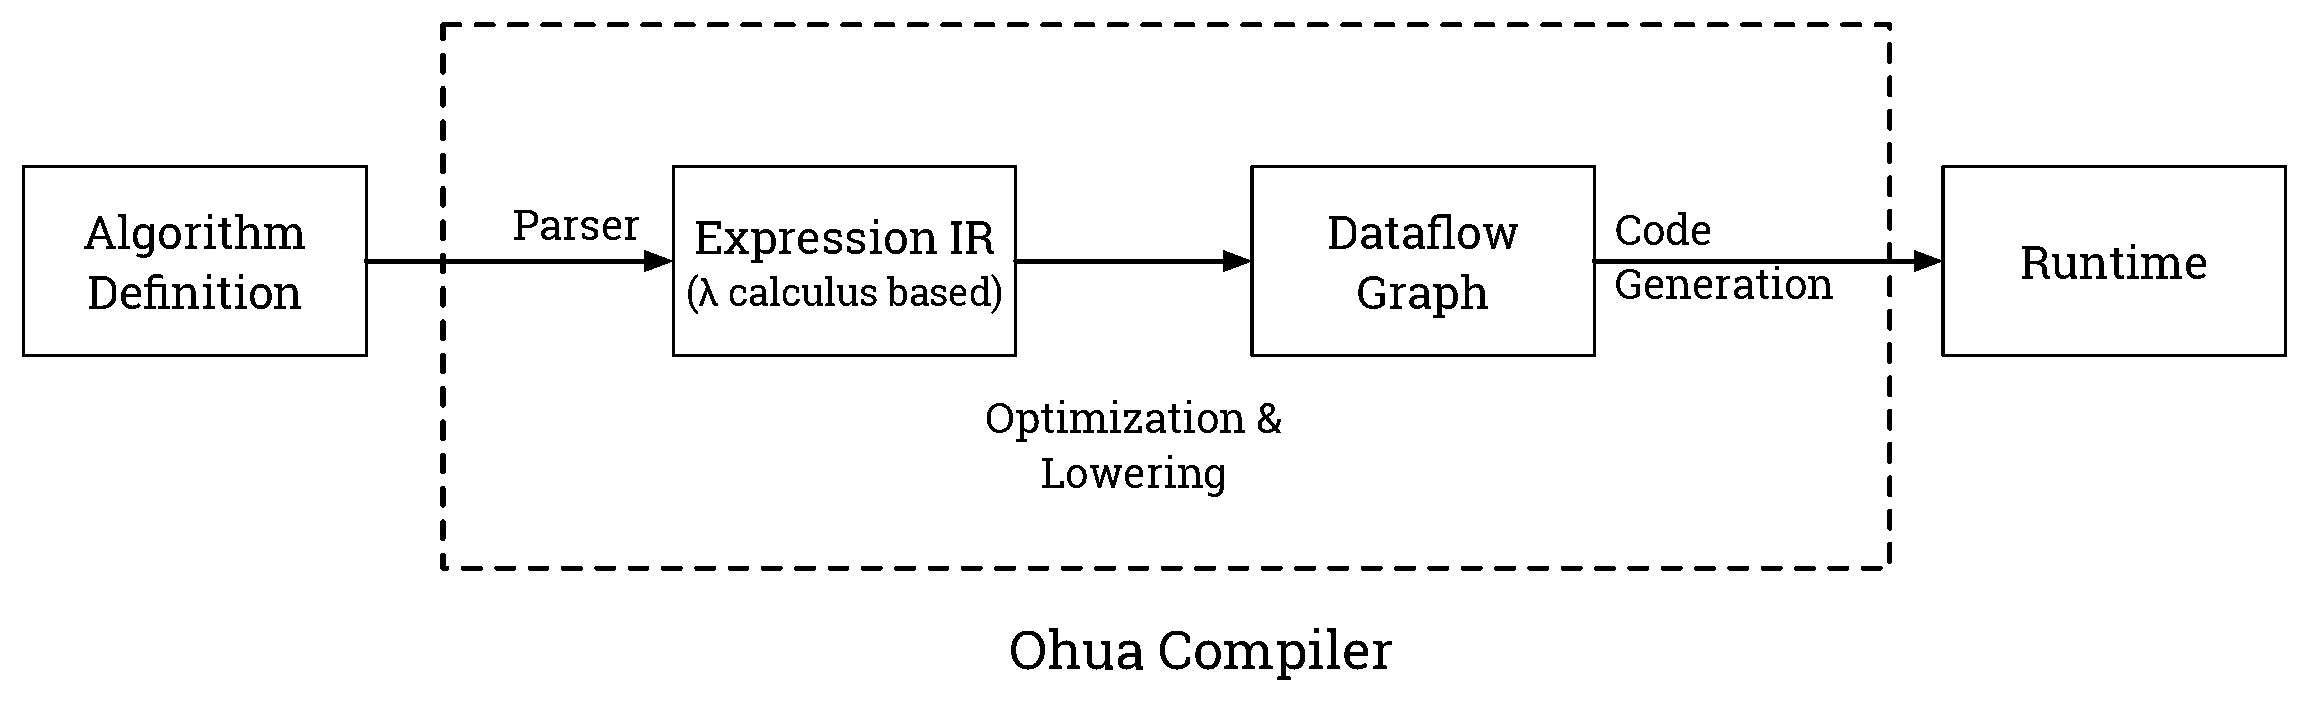
\includegraphics[width=\textwidth,keepaspectratio]{gfx/background-ohua}
    \caption{Overview of the Ohua compiler and its components}%
    \label{fig:background:ohua}
\end{figure}

An Ohua algorithm is what might come closest to the abstractions and tools used by other paradigms.
It describes the part of a program that should be turned into a parallelized runtime.
In early versions~\cite{ertel2015ohua} these algorithms were written in separate files using a high-level language that closely resembled Lisp and OCaml.
Over time, a Rust-like syntax~\cite{adam2019master} had also been added to allow for more imperative algorithm definitions.
By now, algorithms are not separately defined anymore and instead are functions that are written in a host language which is supported by Ohua, such as Rust and Go.
\todo{detail caveats: are there restrictions?}
Ohua comes with a standalone compiler called \rust{ohuac}, which proceeds to parse the algorithm and transforms it eventually into an optimized dataflow graph.
These optimizations stem from a number of transformations that are applied to the dataflow graph to uncover more parallelism opportunities.
A host language specific backend will then generate the runtime code based on the DFG.
This runtime executes as regular part of the program it is embedded in when the algorithm is called.
As such, it may import and use any function from the host code, allowing the developers seamless integration of their existing code into the new parallel algorithm.

Ohua derives parallelism from executing independent nodes of the dataflow graph in parallel (task-level parallelism) and running multiple invocations of dependent nodes in a pipeline-parallel fashion.
In order to rule out most of the common pitfalls in parallel programming, the use of shared state is forbidden in Ohua.
Instead, data must be transferred explicitly by using arguments and function return values.
This also rules out mutable global values which often represent state in programs.
To still allow the convenient declaration of stateful algorithms, Ohua uses the concept of so-called \emph{stateful functions}~\cite{ertel2019stclang}.
A stateful function is a host function that is associated with state values which it is allowed to modify.
Ohua encapsulates this operation and the associated state to ensure it is not leaked or used in a shared fashion.

\begin{figure}[h]
    \begin{subfigure}[h]{.5\textwidth}
        \begin{minted}{Rust}
            let words = vec!["a", "test"];
            let buffer = Buffer::new();
            let _ = for w in words {
                buffer.append(w);
            };
            buffer.get_message();
        \end{minted}
        \caption{Algorithm declaration in Rust}
        \label{fig:backend:smap:algo}
    \end{subfigure}
    \begin{subfigure}[h]{.5\textwidth}
        \missingfigure{Add DFG}
        \caption{The algorithm's dataflow graph. Dependencies in the control flow are dotted.}
        \label{fig:backend:smap:dfg}
    \end{subfigure}
    \caption{Example of an Ohua algorithm using the \rust{smap} primitive.}%
    \label{fig:background:smap}
\end{figure}

Ertel et al.\ additionally proposed \rust{smap}, a stateful map primitive that applies an algorithm to a sequence of items~\cite{ertel2019stclang} and is based on the insight, that loop operations modifying shared state can be considered as fold operations on the state.
An example algorithm in Rust that outlines this is shown in Fig.~\ref{fig:background:smap}.
Functions highlighted in red are builtin functions of the Ohua runtime, all other nodes are host functions provided by the developer.
In our example, the \rust{smap} primitive is represented by the for loop and its use of the \rust{buffer} variable in the body.
The loop body is applied to a sequence of items, just as it would happen in a normal \rust{map} statement.
But additionally, \rust{smap} ensures that changes made to the encapsulated state persist, as they would in a normal \rust{for} loop.
This allows the use of pipeline parallelism for longer loop bodies and -- if no state is used in the loop at all -- the use of data parallelism.
So in Fig.~\ref{fig:background:smap}, the newly initialized buffer is bound to the \rust{append} function, which is called like a method on the state repeatedly for the individual loop iterations.
Any results which would be produced by this loop, are then collected and upon completion of the loop passed on to the next node in the dataflow graph.
In the small code snippet provided, an iteration simply produces a \rust{()} literal\footnote{The \rust{()} type is called Unit literal in Rust. It is the result of a computation that returns nothing and can be compared to the \rust{void} type in C.} and hence the loop result itself is discarded.
What remains, is the side effect of state alteration that occured during the loop processing.
After the loop completes, the next function is executed.
To avoid \rust{get_message} being called too early, a control flow dependency is added to the (otherwise useless) \rust{collect} function.

The result of Ohua's programming model is \emph{deterministic parallelism}, as opposed to Software Transactional Memory which aims to improve execution times by scheduling possibly conflicting operations for parallel execution, completely forfeiting any determinism in the process.
Another advantage is the way in which Ohua is integrated into existing code bases.
In its current version, algorithms are defined as normal functions within the code, allowing developers to first test their implementations without any parallelism before compiling them with Ohua.
This offers the advantage of producing mostly\todo{remove "mostly" when adding no caveats above} framework agnostic code which can be easily reused in other applications as well.
\todo{talk about guarantees compared to stm?}

Challenging however, is the ban the framework places on the use of shared state.
As discussed in chapter~\ref{sec:background:irregular}, many applications encountered in the real world are irregular and hence rely on the use of pointers and shared, global state.
Since Ohua currently only fosters the use of local state with its stateful functions primitives, it is unclear whether it is possible to apply these concepts to shared state programs, which the Software Transactional Memory framework caters towards.


\section{Irregular Applications}
\label{sec:background:irregular}

Providing a comprehensive comparison between STM and Ohua requires a selection of representative applications to test both systems on.
But to make such a selection, one first has to understand, which features describe a parallel application and how these properties may influence the parallel behavior as well as the viability of certain parallelism frameworks.
In the past, most of the research conducted in the field of performance improvements for parallel programs has concerned itself with what is called regular applications.
There are applications, whose degree of exploitable parallelism is simply determined by the program structure and the size of the input set.
As both of there properties are known or can be inferred at compile time, any optimization potential is easy to uncover and exploit for compilers.

When looking at \emph{irregular applications} on the other hand, the situation is completely different.
The term describes applications, whose structure resolves around the manipulation of large, pointer-based data structures like graphs and trees.
Due to this structural peculiarity, compiler analyses struggle to uncover any meaningful insights into the algorithm that would allow to exploit any parallelism hidden in it.

\begin{figure}[b]
    \centering
    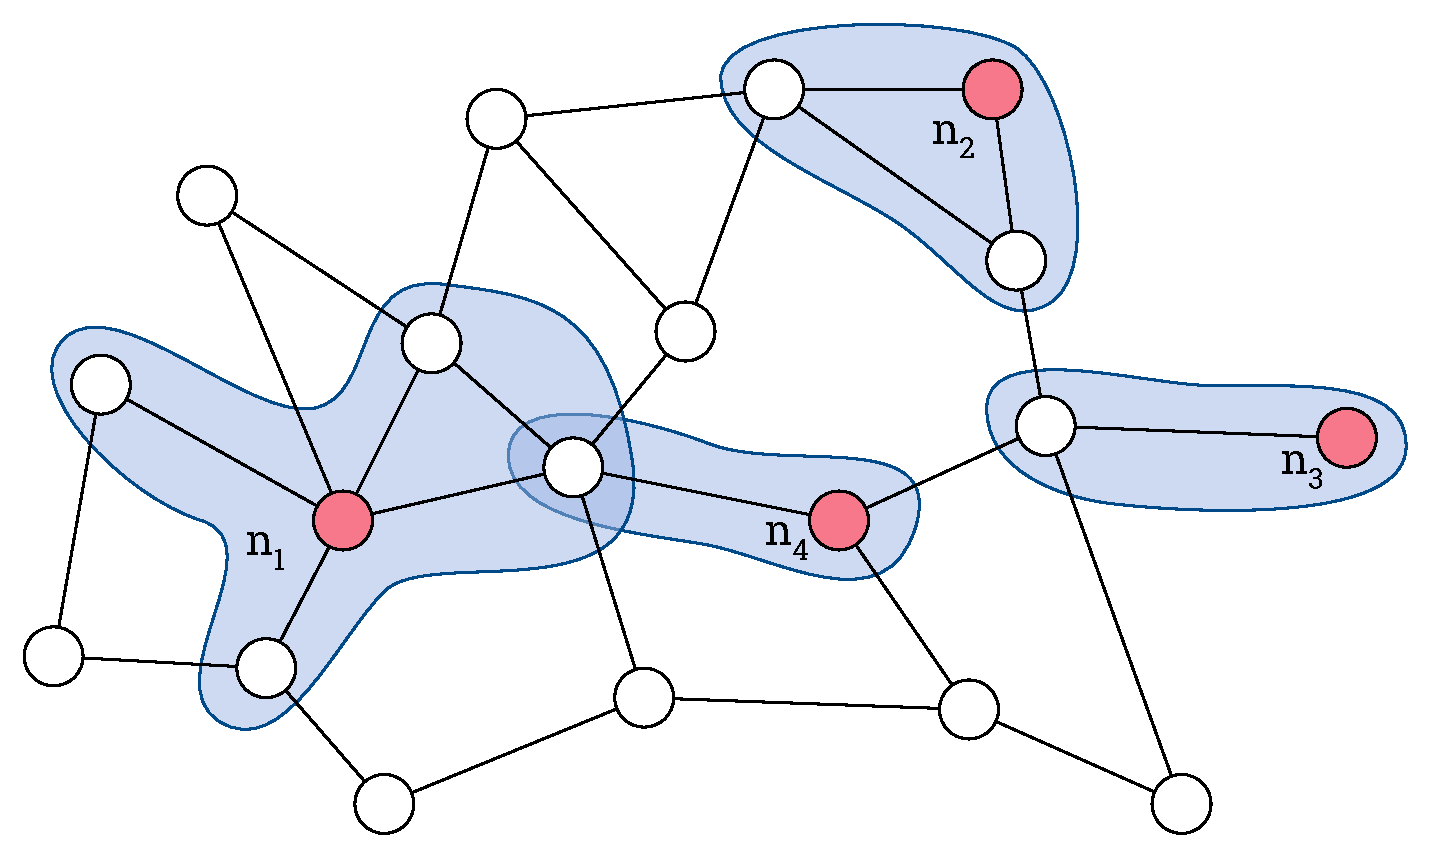
\includegraphics[width=.7\textwidth,keepaspectratio]{gfx/background-irregular}
    \caption{Graph representation of an irregular application with active elements and their neighborhoods. Adapted from Kulkarni et al.~\cite{kulkarni2009much}}%
    \label{fig:background:irregular}
\end{figure}

To better outline this, Kulkarni et al.~\cite{kulkarni2009much} developed an abstract representation for irregular programs using a set of nodes and edges, as shown in Fig.~\ref{fig:background:irregular}.
The nodes and edges represent the input data and their relationships.
During the execution of an irregular algorithm, the program may perform computations on a (sub-)set of active nodes or edges, the work items.
In Figure~\ref{fig:background:irregular}, these are highlighted in red.
Performing said executions may involve reading from or writing to other nodes or edges in the graph, which form an active elements' neighborhood, shaded in blue.
Which elements of the graph make up the neighborhood of an active element is not known beforehand and may encompass all direct neighbors in the graph (as seen for nodes $n_2$ and $n_3$), maybe only a single neighboring element (as seen for node $n_4$) or transitively the neighboring elements of its direct neighbors.

Usually, work items are not ordered and may be processed in any order.
But processing one element may generate an arbitrary number of new active elements or remove others from the pool, depending on the algorithm.
Also, some active elements may not be processed simultaneously due to overlapping neighborhoods, as the changes made by processing both items may conflict with each other.

Since all these relationships and interdependencies are not known beforehand but rather depend on the input data, this information cannot be uncovered and used by compile time analyses.
And because static parallelization as well as lock-based approaches fail to uncover any viable parallelism opportunities in these programs, Kulkarni et al.~\cite{kulkarni2007optimistic} argue, that optimistic strategies such as \emph{Software Transactional Memory} need to be used to tackle this class of problems.
This is because, as we have shown, the heavy use of pointers in the program hinders efficient analyses but as conflicts due to parallelization may be rare (depending on the input data) the optimistic trial-and-abort semantics of STM allow for a simple and efficient parallelization in most cases.\todo{Kommt hier gut genug raus, warum diese Section hier in der Arbeit steht? Also: Zusammenhang ADP/IA klar?}
As of now, it is unclear whether Ohua could also be used to parallelize Irregular Applications, offering an alternative besides STM for this type of applications where most other frameworks fail.
Since its approach relies heavily on compile-time analyses and optimizations, it may prove challenging to try to uncover good parallelism opportunities here.


\subsection{Amorphous Data Parallelism}
\label{sec:background:irregular:adp}

Pingali et al.~\cite{pingali2009amorphous} argue, that most irregular applications additionally exhibit a behavior referred to as \emph{amorphous data parallelism}:

Given a set of active nodes and an ordering on them, amorphous data parallelism is the parallelism that arises from simultaneously processing active nodes and is subject to neighborhood and ordering constraints.
It is a generalization of standard data parallelism in which
\begin{enumerate}
    \item concurrent operations may conflict with each other
    \item activities can be created dynamically
    \item activities may modify the underlying data structure
\end{enumerate}
These characteristics have already been briefly discussed in connection with Fig.~\ref{fig:background:irregular}.

While irregular applications are hard to reason about due to their pointer usage, they are still a very interesting research topic, made more difficult by amorphous data parallelism.
But as we will show in chapter~\ref{sec:experiments}, applications of this type are common and widespread in different aspects of real world applications.




% - present both Ohua and STM
%   - explain paradigms in detail (most people here don't know what stm is and how it works!)
%   - detail benefits and shortcomings of both
%   - Ohua: talk about the compiler, its stages and where optimizations hook in as this will be required information later on.
%   - STM: Detail that non-determinism is part of the execution model -> speculative parallelism
%       - make sure to thoroughly explain the concept of a transaction
%   - Ohua: detail determinism of the model if appropriate, but remember that this will also be discussed later on
% - explain Irregular Applications: They are different from the parallelizability problems we usually face as the input dictates the parallelism at runtime and the computing times!
%   - use: \label{sec:background:irregular}

% !TEX root = ../thesis.tex
%
\chapter{Preliminary Studies}
\label{sec:preliminary}

In order to determine the usability of Ohua for implementing shared state applications and to identify any necessary modifications to the compiler or the runtime, we first tried to implement a single such application with it.
After successful implementation we wanted to compare its performance against a Software Transactional Memory implementation of the same program and see, whether there are any shortcomings of Ohua in terms of performance.
Based on this initial study we then wanted to find ways to improve Ohua's performance, if necessary, e.g., by introducing new compiler optimizations.
The aim of these preliminary studies was to find out, whether Ohua was usable for writing programs relying on shared state and if it could be a viable alternative to STM in this setting.

\section{Labyrinth Benchmark}

As a first example application, we chose to implement the \emph{labyrinth} benchmark as presented by Swalens et al.~\cite{swalens2016transactional}.
This algorithm is a variation of Lee's Algorithm~\cite{lee1961algorithm} which solves path-connection problems often encountered when searching for an optimal route or generating wiring diagrams where wires may not overlap.
We base our own implementation on the descriptions of Watson et al.~\cite{watson2007study}, who presented an implementation for Transactional Memory.

\begin{figure}[b]
    \begin{subfigure}[t]{.24\textwidth}
        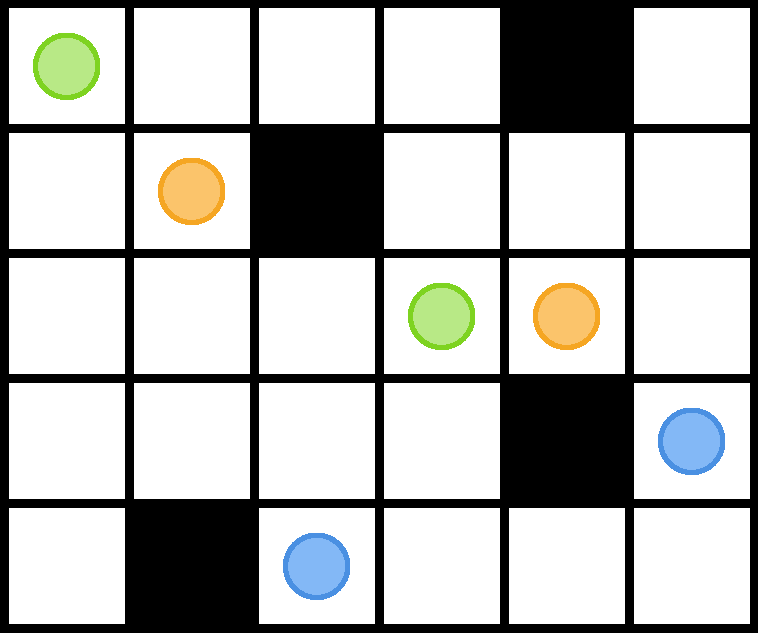
\includegraphics[width=\textwidth,keepaspectratio]{gfx/preliminaries-labyrinth/1-maze_points}
        \caption{Initial grid with 3 point pairs.}%
    \end{subfigure}%
    ~
    \begin{subfigure}[t]{.24\textwidth}
        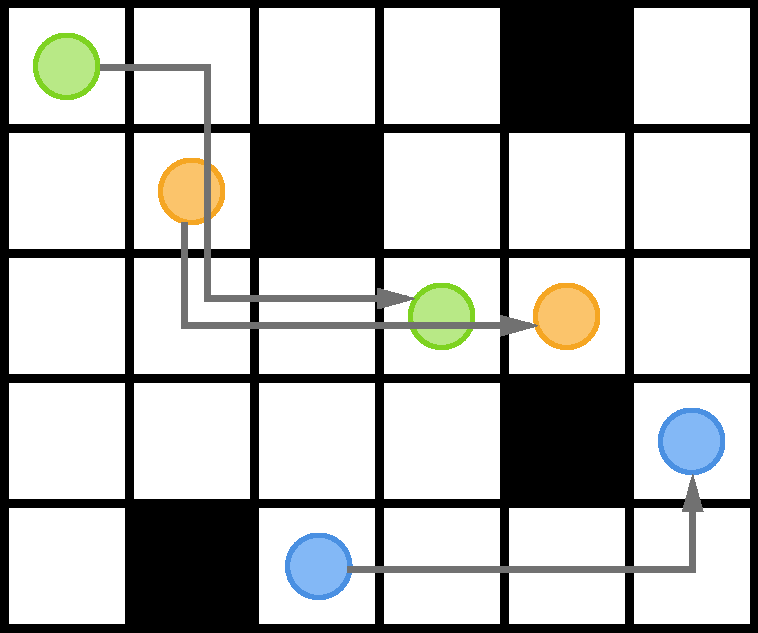
\includegraphics[width=\textwidth,keepaspectratio]{gfx/preliminaries-labyrinth/2-maze_paths}
        \caption{Possible paths between the points.}%
    \end{subfigure}%
    ~
    \begin{subfigure}[t]{.24\textwidth}
        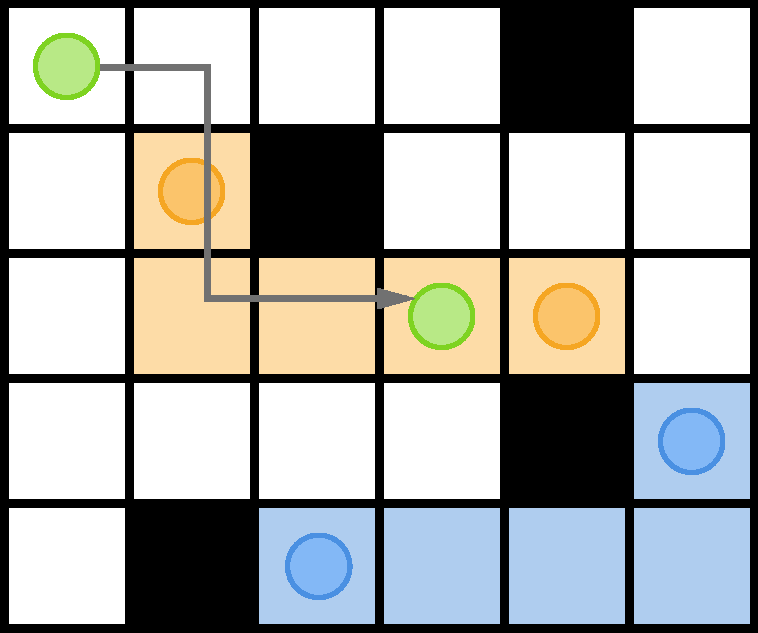
\includegraphics[width=\textwidth,keepaspectratio]{gfx/preliminaries-labyrinth/4-maze_update2}
        \caption{First two paths are mapped into the maze.}%
    \end{subfigure}%
    ~
    \begin{subfigure}[t]{.24\textwidth}
        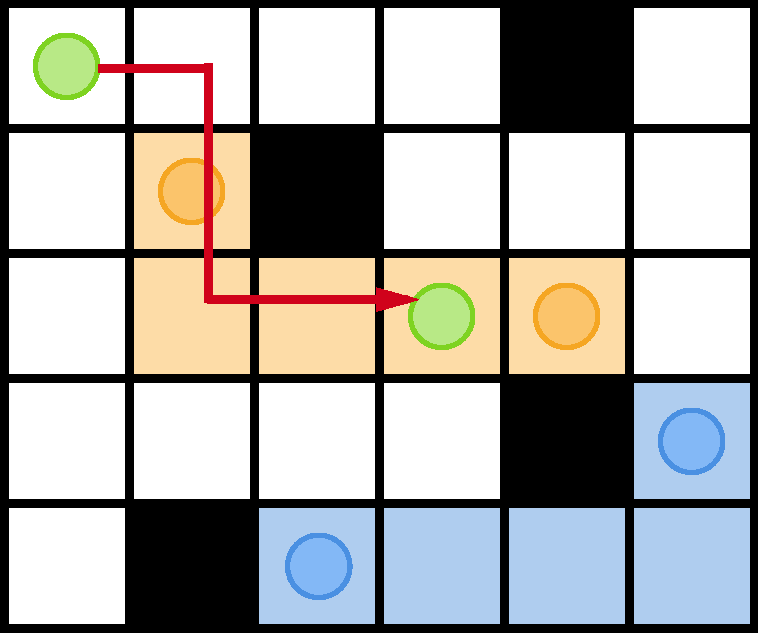
\includegraphics[width=\textwidth,keepaspectratio]{gfx/preliminaries-labyrinth/5-maze_update3}
        \caption{Conflict for the third path as it goes through a now-occupied segment.}%
        \label{fig:preliminary:labyrinth:unroutable}
    \end{subfigure}%
    \caption{Illustration of the operation of the labyrinth benchmark, showing the (attempted) mapping of 3 paths in a 6 $\times$ 5 two-dimensional grid. Black squares represent walls that cannot be routed through.}%
    \label{fig:preliminary:labyrinth}
\end{figure}

Goal of the benchmark is to find a number of paths within a three-dimensional maze, as depicted in Fig.~\ref{fig:preliminary:labyrinth}.
As input, the algorithm is provided with a maze and a set of pairs of points, between which a path is to be found and mapped within the maze.
During execution, one pair of coordinates is removed from the list of points (the worklist) and the program attempts to find a path between both points in the maze.
This is done using a breadth-first search.
The maze itself may also contain \enquote{walls} (highlighted as black squares in Fig.~\ref{fig:preliminary:labyrinth}), through which no path can be routed.
Also, each point in the maze may only be occupied by a single path to rule out overlapping paths.
The algorithm terminates once the worklist is empty and all paths have either been mapped successfully or deemed unmappable by the absence of a valid connection between both points.

This benchmark is a classic example for an \emph{irregular application}: all operations happen on the shared maze data structure which is modified in the process.
Additionally, any data parallelism obtainable in the application is \emph{amorphous}, as mapping one path in the maze may render another pair of coordinates unroutable as both points get cut off from one another.
An example for this can be seen in Fig.~\ref{fig:preliminary:labyrinth:unroutable}, where the mapping of the orange path makes finding a path between the green coordinates impossible as one point is part of the orange path.
As we have learned in chapter~\ref{sec:background:irregular}, this specific class of problems can be parallelized easily using Software Transactional Memory.
Searching for a single path can be compartmented into a transaction, treating all maze fields as transaction variables.
Listing~\ref{fig:preliminaries:stm} shows the resulting transactional implementation of the labyrinth benchmark.

\begin{listing}[t]
    \begin{minted}[fontsize=\footnotesize]{Rust}
        let (worklist, grid) = /* read from file */

        for points in worklist {
            atomically(|trans| {
                let local_grid = create_working_copy(&grid);

                if let Some(path) = find_path(points, &local_grid) {
                    // if path is found, write back results
                    update_grid(&grid, &path, trans)?;
                }

                Ok(())
            });
        }
    \end{minted}
    \caption{Simple implementation of the labyrinth benchmarks using Software Transactional Memory in Rust.}%
    \label{fig:preliminaries:stm}
\end{listing}

All path pairs are collected in a worklist, through which the algorithm iterates (line 3).
Inside the transaction that is started for each item (line 4), a working copy of the maze is created as detailed in~\cite{swalens2016transactional} to reduce the number of repeated reads from individual transaction variables.
Then, the breadth-first search commences in order to discover a route between the starting point and the target (line 7).
Note that since we've made a copy of the grid beforehand, this happens completely locally.
When a path is found, an update is run on the grid, inserting the path (line 9).
Should another transaction, which also happened to alter one or more segments of the newly-found path, manage to commit in the meantime, the resulting conflict is detected and the transaction is rolled back and re-run until either the update commits successfully or no path can be found anymore.
Our transactional memory implementation is a mere adaption of the algorithm outlined above, augmented with concurrency by splitting the worklist into $n$ parts, which are processed by $n$ threads in parallel.

In our first Ohua implementation, we described idiomatically, what the algorithm should be doing.
Listing~\ref{fig:preliminaries:ohua1} shows this simple program: First, all paths are searched for individually (lines 2-4), before they are written to the grid (line 6).
If a path conflicts with a previously saved one (i.e., at least one segment of the path is not free anymore), it is scheduled for re-computation by adding it to the \rust{remap_paths} vector.
Until all paths have either been mapped or discarded as unroutable, these steps are repeated recursively, although this invocation has been omitted from the sample code for the sake of simplicity.

\begin{listing}[t]
    \begin{minted}[fontsize=\footnotesize]{Rust}
        fn fill(maze: Maze, to_map: Vec<(Point, Point)>) -> Maze {
            let paths = for pair in to_map {
                find_path(maze, pair)
            };

            let (remap_paths, new_maze) = update_maze(maze, paths);

            // recursively call `fill` as necessary
        }
    \end{minted}
    \caption{Simplified first implementation of an recursive Ohua algorithm for the labyrinth benchmark}%
    \label{fig:preliminaries:ohua1}
\end{listing}

This implementation resembles an executable version of an Ohua algorithm that did compile and run with the initial Ohua compiler framework.\todo{Clarify distinction between Ohua versions: Which is default?}
In contrast to the STM algorithm, the maze update has been moved out of the inner loop, since this operation should remain sequential, following Ohua's idea of fostering local state, as introduced in chapter~\ref{fig:background:ohua}.

% TODO: Maybe subsection?
\subsection{First Results}

To establish a baseline for performance comparison, we measured the execution time of both benchmarks and calculated the speedup in relation to a sequential implementation, as outlined in chapter~\ref{sec:experiments:measurements}.
In an attempt to achieve comparable results, we used the same input data that had also been used previously by other authors and was originally proposed by Minh et al.~\cite{minh2008stamp}.
The chosen input maze for our test run had a size of 128 $\times$ 128 $\times$ 5 cells and required the mapping of 128 paths, given as predefined coordinate pairs, into it.
Resulting speedup figures for a varying number of worklist splits are shown in Fig.~\ref{fig:preliminaries:initial-results}.

\begin{figure}[h]
    \centering
    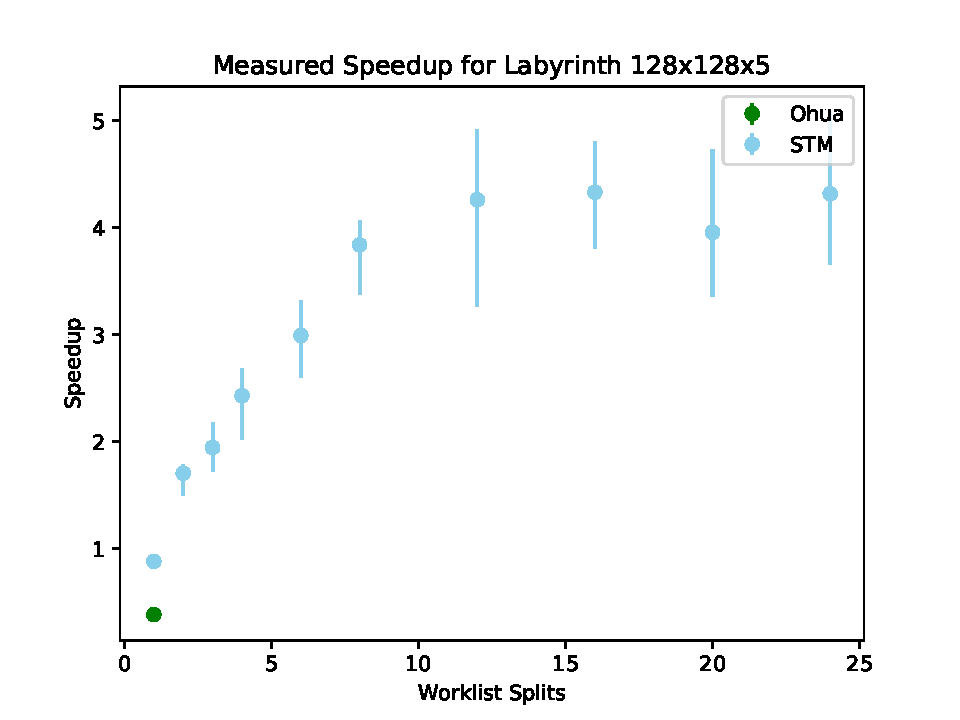
\includegraphics[width=.5\textwidth,keepaspectratio]{gfx/preliminaries-labyrinth/2019-04-18-128x128x5}
    \caption{Measured speedups of the labyrinth application for the STM and Ohua implementations.}%
    \label{fig:preliminaries:initial-results}
\end{figure}

As one can see in the plot, Software Transactional Memory is able to achieve a logistic growth for its speedup for 1 to 24 worklist splits, which converges at a mean maximum speedup of about 4.3.
Ohua on the other hand recorded only a single measuring point for a run with no worklist splitting at all.
This single run exhibited a speedup of less than 0.5, meaning it took more than twice as long to complete as the sequential reference implementation.
The reason for this is the absence of any configuration options for e.g. worklist splits.
Hence, there is no data parallelism in the Ohua algorithm, as the Rust runtime does not support parallel loops yet.
Effectively, this single measurement shows the performance of a sequential algorithm executed with the Ohua runtime, revealing the overhead it has compared to a normal sequential implementation.
Most of the overhead stems from the spawning of the threads each operator lives in and the resulting movement of data between these threads.\todo{Maybe produce a diagram showing the overhead in comparison?}
Our hope is to show that these overheads amortise with increased data parallelism.

In order to achieve more data parallelism and an overall improved performance, we were looking for modifications that could be made to the Ohua algorithm to accomplish this.
We first wanted to introduce manual changes to the algorithm without making amendments to the compiler to test different approaches easily.
These manual changes simply emulate the changes a compiler pass would make on the algorithm layer.
After identifying the optimizations that indeed provide a performance boost, we generalized them into compiler optimizations applicable to all algorithms.
The resulting transformations will be discussed in chapter~\ref{sec:transformations}.


\section{Parallel Loop Implementation}

As Fig.~\ref{fig:preliminaries:initial-results} clearly showed, the most pressing issue with the existing Ohua implementation for Rust was the absence of any data parallelism facilities like parallel loops.
Our first assumption based on these results was, that most performance could be gained simply by processing multiple labyrinth paths in parallel, as this operation makes up for most of the execution time in the sequential implementation.\todo{Show graphics that outline what takes how long. Take data from flamegraph}
The idea was to split the worklist into $n$ equally sized chunks and process them in parallel, which is similar to what STM does.
Listing~\ref{fig:preliminaries:ohua2} shows an exemplary implementation for an algorithm splitting the worklist in two parts.
Lines that were changed compared to the previous iteration are highlighted.

\begin{listing}[b]
    \begin{minted}[fontsize=\footnotesize,highlightlines={2-10}]{Rust}
        fn fill(maze: Maze, to_map: Vec<(Point, Point)>) -> Maze {
            let (tm0, tm1) = splitup(to_map);
            let part0 = for pair in tm0 {
                find_path(maze, pair)
            };
            let part1 = for pair in tm1 {
                find_path(maze, pair)
            };

            let paths = join(part0, part1);

            let (remap_paths, new_maze) = update_maze(maze, paths);

            // recursively call `fill` as necessary
        }
    \end{minted}
    \caption{Labyrinth implementation in Ohua using worklist splits for parallelism.}%
    \label{fig:preliminaries:ohua2}
\end{listing}

The main difference to the previous iteration of the algorithm is the introduction of two new operators, \rust{splitup} and \rust{join}.
These are implemented in the user space for this example but would become part of the runtime when this alteration is translated into a compiler transformation.
Their task is simply to split the worklist up into the required number of parts and merge them back together, once results have been produced.
Data parallelism is introduced in a very verbose manner by the duplication of the loop (lines 3-8).
This change can be scaled for an arbitrary number of threads by partitioning the worklist into as many parts as necessary for testing purposes.

% discuss the effect of this change (i.e., did it work? graph!)
Introducing a rudimentary form of data parallelism helped not only to obtain multiple meaningful measurements for Ohua, but also led to better performance, as can be seen in Fig.~\ref{fig:preliminaries:split-results}.
It now also exhibits a performance growth behavior that can roughly be described as logistic, though it only manages to achieve half as much speedup as STM.
Upon investigating this performance gap we determined two fundamental problems resulting from our current algorithm: Retries and Stragglers.

%\begin{figure}[h]
    %\centering
    %\begin{minipage}{.5\textwidth}
        %\centering
        %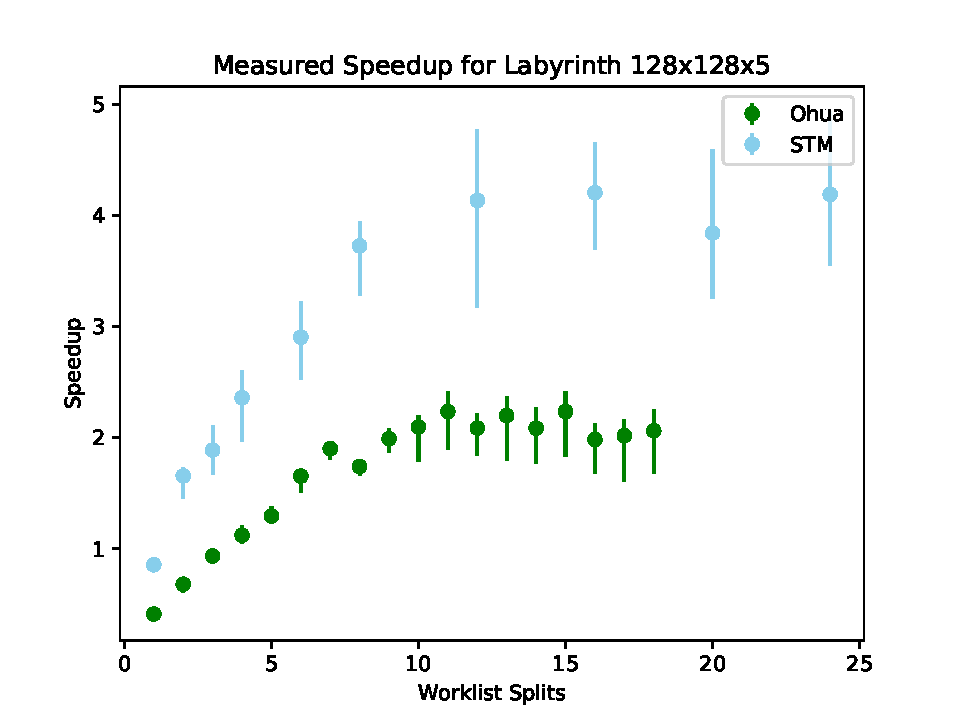
\includegraphics[width=.95\linewidth,keepaspectratio]{gfx/preliminaries-labyrinth/split_128x128x5}
        %\captionof{figure}{Measured speedup for an Ohua implementation using worklist splits.}%
        %\label{fig:preliminaries:split-results}
        %\vfill
    %\end{minipage}%
    %\begin{minipage}{.5\textwidth}
        %\centering
        %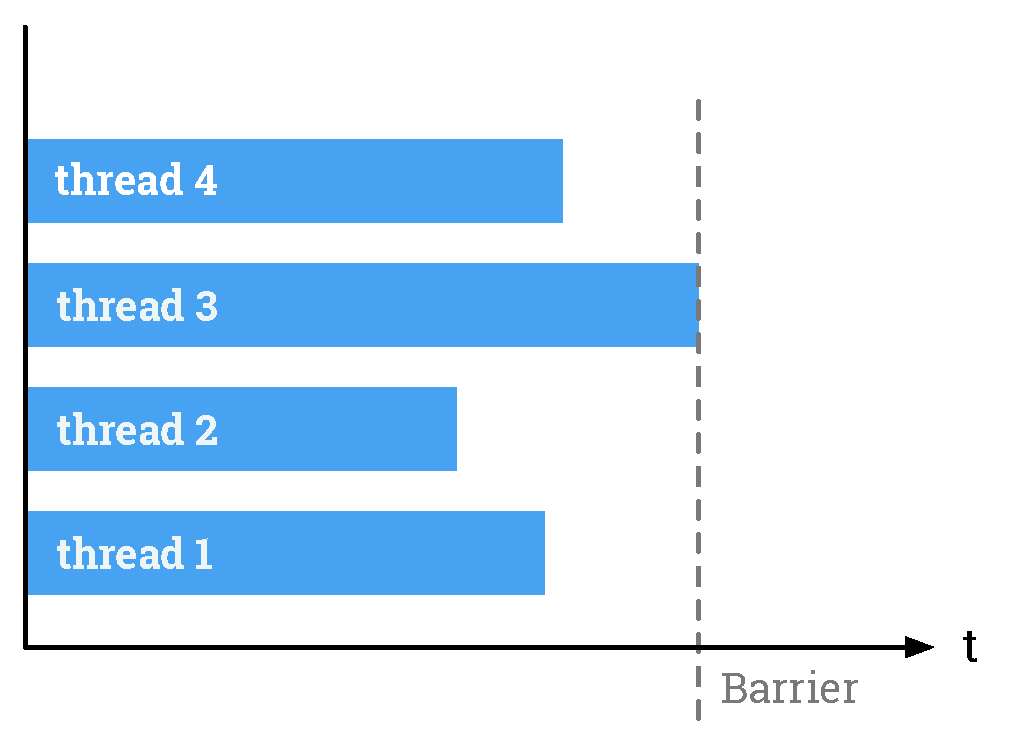
\includegraphics[width=.95\linewidth,keepaspectratio]{gfx/preliminaries-labyrinth/preliminaries-straggler}
        %\captionof{figure}{Visualization of the straggler problem. Thread 3 takes the longest to finish its assigned work set, forcing the others to idle.}
        %\label{fig:preliminaries:stragglers}
    %\end{minipage}
%\end{figure}

\begin{figure}[h]
    \centering
    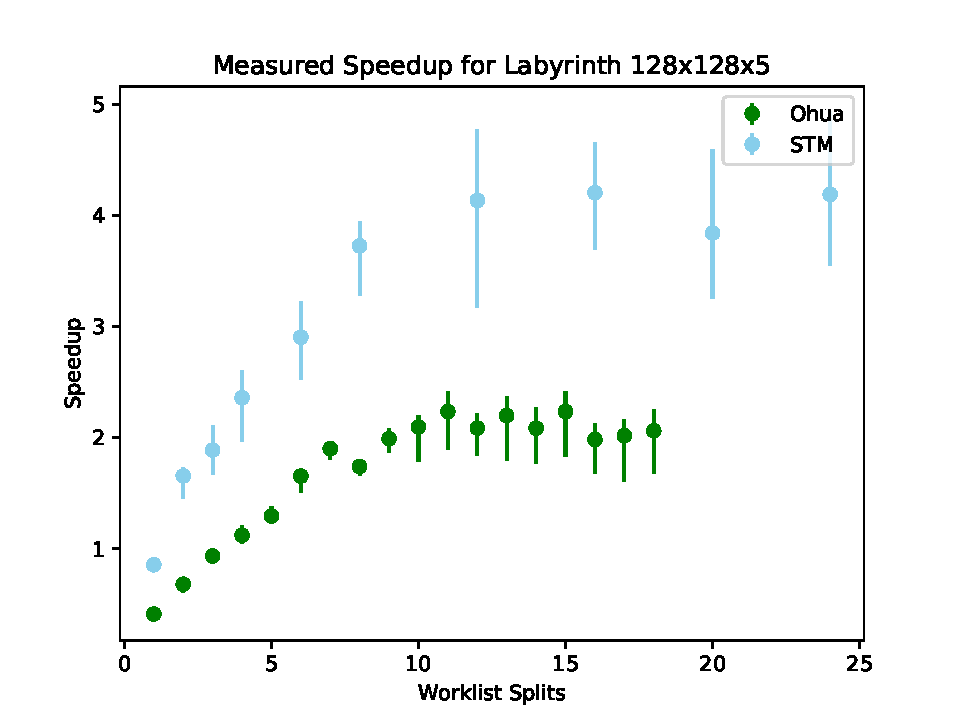
\includegraphics[width=.5\textwidth,keepaspectratio]{gfx/preliminaries-labyrinth/split_128x128x5}
    \caption{Measured speedup for an Ohua implementation using worklist splits.}%
    \label{fig:preliminaries:split-results}
\end{figure}

Besides data parallelism, another important factor influencing the execution time of the benchmark\footnote{In fact, this holds true for any irregular application following this \emph{Calculate-Update Pattern}.} is the number of repeated calculations that is necessary.
As described before, the labyrinth benchmark is designed to repeatedly attempt to find a route between each coordinate pair until a path is either successfully mapped or no valid path can be found anymore.
In the sequential implementation, this is not an issue as each path is searched for and updated individually without any concurrency, guaranteeing that each coordinate pair will only ever be evaluated once.
Any concurrent implementation however, comes at the cost of potential write conflicts that need to be resolved.
STM for example uses $n$ threads, always working on finding $n$ paths in parallel which are then written to the maze.
This means that from the perspective of one thread, in between its last access to the maze and an attempted update, about $n - 1$ changes will ideally have been made to the maze, each possibly introducing a conflict provoking a recomputation of the given path.
So at worst, per iteration of $n$ threads, $n-1$ results may become invalid due to a write conflict, forcing recomputation.\\
For Ohua, this number is significantly higher.
Its current approach is to update the shared state as late as possible, after computing all paths.
The negative side effect of this is that in a run to map $p$ paths, $p-1$ results may require a recomputation per recursion step in the worst case, possibly leading to as much as $\sum_{0 \leq i < p} i$ conflicts, which may in part explain the bad performance of Ohua.\todo{Maybe add some data about retries? (Numbers for Ohua and STM)}

The second relevant performance bottleneck is the straggler problem.
In research, when reasoning about parallel tasks it is often assumed that all tasks perform uniformly, i.e., require the same time to complete.
Real applications however rarely fulfill this assumption.
On the contrary, the tasks in these worklists are often wildly heterogeneous, each requiring a different amount of processing time.
This is also the case in the labyrinth benchmark.
The processing time for a single path depends solely on the number of nodes the path finder has to inspect which is related to the distance between the starting coordinates and the target.
As result, the $n$ threads of our algorithm each take differently long to process their worklist, which means that all threads finishing their work earlier have to wait at the synchronization point for all slower threads to finish.
This forced slack time is also present in the STM algorithm implementation, yet not as severe as in the Ohua implementation, since it synchronizes all threads only once when terminating them, while Ohua's threads synchronize once per recursion step.


\section{Lowering the Retry Count}
\label{sec:preliminaries:retries}

\begin{listing}[!b]
    \begin{minted}[fontsize=\footnotesize,highlightlines={2,14}]{Rust}
        fn fill(maze: Maze, to_map: Vec<(Point, Point)>, frequency: usize) -> Maze {
            let (points, still_to_map) = take_n(to_map, frequency);
            let (tm0, tm1) = splitup(points);
            let part0 = for pair in tm0 {
                find_path(maze, pair)
            };
            let part1 = for pair in tm1 {
                find_path(maze, pair)
            };
        
            let paths = join(part0, part1);
        
            let (remap_paths, new_maze) = update_maze(maze, paths);
            let to_remap = join(remap_paths, still_to_map);
        
            // recursively call `fill` as necessary
        }
    \end{minted}
    \caption{Ohua algorithm using a fixed update frequency to lower the number of write conflicts.}%
    \label{fig:preliminaries:ohua3}
\end{listing}

Initially, we abandoned the idea of updating the maze after every state update in favor of a single update after processing all elements, to attempt solving the problem using only local state and a simple algorithm structure.
Alas, these frequent updates are key to keep the execution time low because the quick propagation of changes ensures that fewer computations are carried out based on outdated information.
Therefore, we altered the algorithm such that updates to the shared state are conducted after processing a fixed number of elements, which we will refer to as the \emph{update frequency} $f$.
In our algorithm, which is shown in Fig.~\ref{fig:preliminaries:ohua3}, this is reflected by introducing a new operator, \rust{take_n}.
Making use of the existing recursion semantics, it caps the number of elements to process per step to at most $f$ elements (line 2).
As before, all computations in a single step are conducted on the same state and updated all at once after finishing mapping the paths.
Once the updates have been written to the maze or rejected due to a collision, the list of failed updates gets merged again with the rest of the worklist that has not been processed in this recursion step (line 14).
Using this approach, the number of possibly denied state updates is dramatically reduced to only maximally $f - 1$ elements.
This has the side effect of reducing the overall probability of a write conflict occurring with decreasing values for $f$.

\todo{Discuss the results from this: Which frequencies are optimal? What measurements did I take? Graph?}
In addition to the number of worklist splits, this change introduced the \emph{frequency} $f$ as second parameter to the algorithm, which we wanted to fix to a specific value to find a middle ground between processing as many elements as possible and keeping the number of retries low.
Small update frequencies imply fewer conflicts, but also more recursions and hence more negative side effects from stragglers.
Choosing a too large value for $f$ on the other hand might improve the parallel performance but comes at the cost of more repeated calculations.
We tested our implementation with varying update frequencies and determined that $f = 2 \cdot threadcount$ provided the best trade-off.
\todo{Generalizability?}


\section{Improving Resource Utilization}
\label{sec:preliminaries:futures}

Stragglers are a common problem in applications processing data in parallel.
Hence, a lot of solutions have been proposed already to tackle this problem using different techniques.
One solution to this problem are work-stealing scheduling strategies, which have been discussed as early as 1981 by Burton and Sleep~\cite{burton1981executing} and later by Halstead~\cite{halstead1984implementation}.
The basic idea of a traditional work-stealing scheduler is that each processor in a computer system is assigned a set of work items to process.
Each item consists of an isolated stream of instructions that is executed, possibly spawning new items in the process.
Work items are unordered and may be processed in any order and in parallel.
Should a processor run out of work, it can \enquote{steal} work items from other queues to avoid idle time.
This concept has also been implemented in software, usually providing a runtime consisting of a thread pool, a scheduler and a set of tasks.
Fig.~\ref{fig:preliminary:straggler} sketches how this approach could reduce the slack time for all threads in a system by stealing work from the longest-running thread.
By reducing the time all threads spend idling, the overall execution time and efficiency improve.

\begin{figure}[h]
    \begin{subfigure}[t]{.45\textwidth}
        \centering
        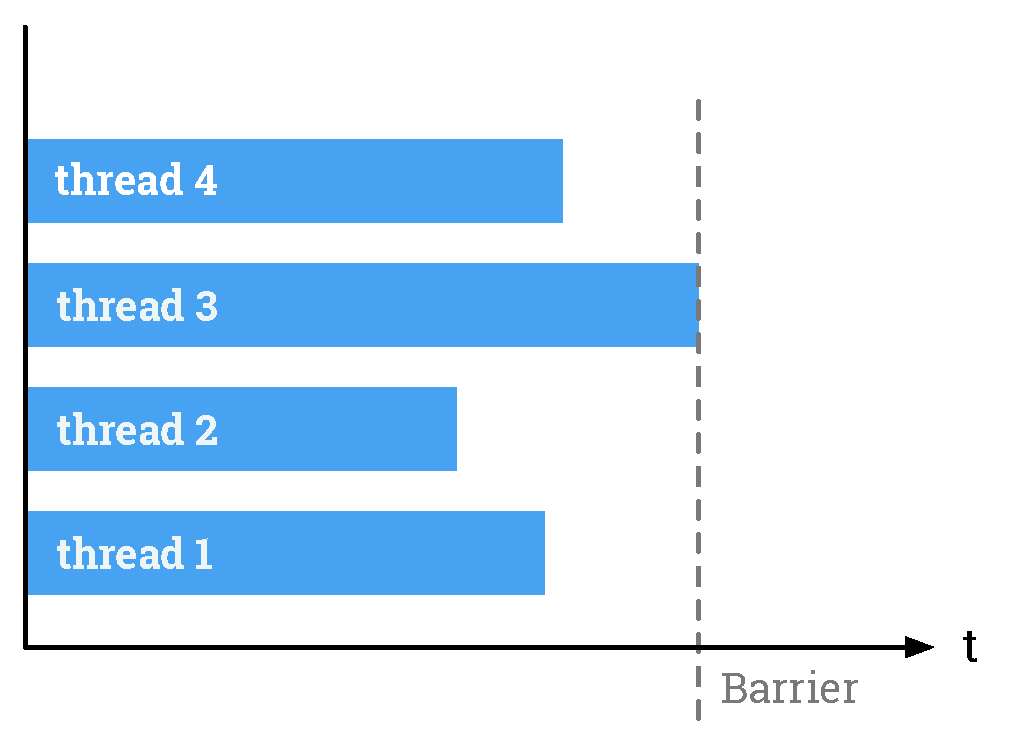
\includegraphics[width=.85\textwidth,keepaspectratio]{gfx/preliminaries-labyrinth/preliminaries-straggler}
    \end{subfigure}%
    \hfill
    \begin{subfigure}[t]{.45\textwidth}
        \centering
        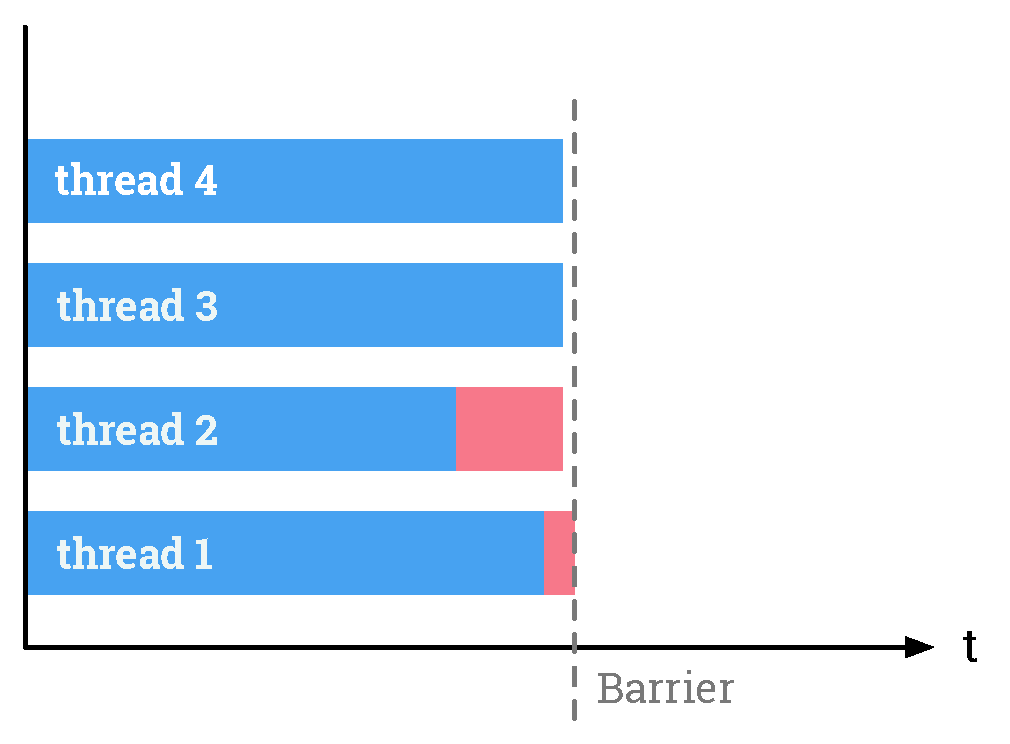
\includegraphics[width=.85\textwidth,keepaspectratio]{gfx/preliminaries-labyrinth/preliminaries-work-stealing}
    \end{subfigure}%
    \caption{Illustration of the straggler problem and how work-stealing scheduling can significantly reduce this problem. In the second illustration, the slack time is almost completely removed by threads 1 and 2 stealing work from thread 3.}%
    \label{fig:preliminary:straggler}
\end{figure}

To mitigate our straggler problem, we decided to move all data-parallel processing to a work stealing runtime.
Rust's ecosystem offers multiple well-matured runtimes for this purpose.
We chose to use \emph{tokio}~\cite{WEB:tokiors2020} as it was the most popular runtime at the time we implemented this, but we kept the code mostly library-agnostic to make a later switch in libraries as easy as possible.

Listing~\ref{fig:preliminaries:ohua4} shows the Ohua algorithm after adding the work-stealing runtime.
Now, its setup in the algorithm \rust{run_algo} (line 2) forms the initial step before running any part of the algorithm itself.
This runtime is then reused throughout all recursion steps of \rust{fill} to keep the added overhead low.
Similar to previous iterations, $f$ items are first taken from the worklist and then split for processing (lines 8-10).
These work sets are then scheduled as tasks for execution on the threadpool (line 11).
Following the findings of Ousterhout et al.~\cite{ousterhout2013case} we make individual tasks as small as possible, each consisting of only a single coordinate pair for optimal load balancing between all threads.
After collecting the results from the runtime (line 12), the algorithm will proceed as in previous versions.

\begin{listing}[t]
    \begin{minted}[fontsize=\footnotesize,highlightlines={1-5,10-12}]{Rust}
        fn run_algo(maze: Maze, to_map: Vec<(Point, Point)>, frequency: usize, threadcount: usize) -> Maze {
            let rt = create_runtime(threadcount);

            fill(maze, to_map, frequency, threadcount, rt)
        }

        fn fill(maze: Maze, to_map: Vec<(Point, Point)>, frequency: usize, threadcount: usize, rt: Arc<Runtime>) -> Maze {
            let (points, still_to_map) = take_n(to_map, frequency);

            let worklist = split_evenly(points, taskcount);
            let task_handles = spawn_onto_pool(worklist, maze, rt);
            let paths = collect_work(task_handles);
        
            let (remap_paths, new_maze) = update_maze(maze, paths);
            let to_remap = join(remap_paths, still_to_map);
        
            // recursively call `fill` as necessary
        }
    \end{minted}
    \caption{Ohua algorithm using a work-stealing runtime to schedule its tasks.}%
    \label{fig:preliminaries:ohua4}
\end{listing}

\begin{figure}[b]
    \centering
    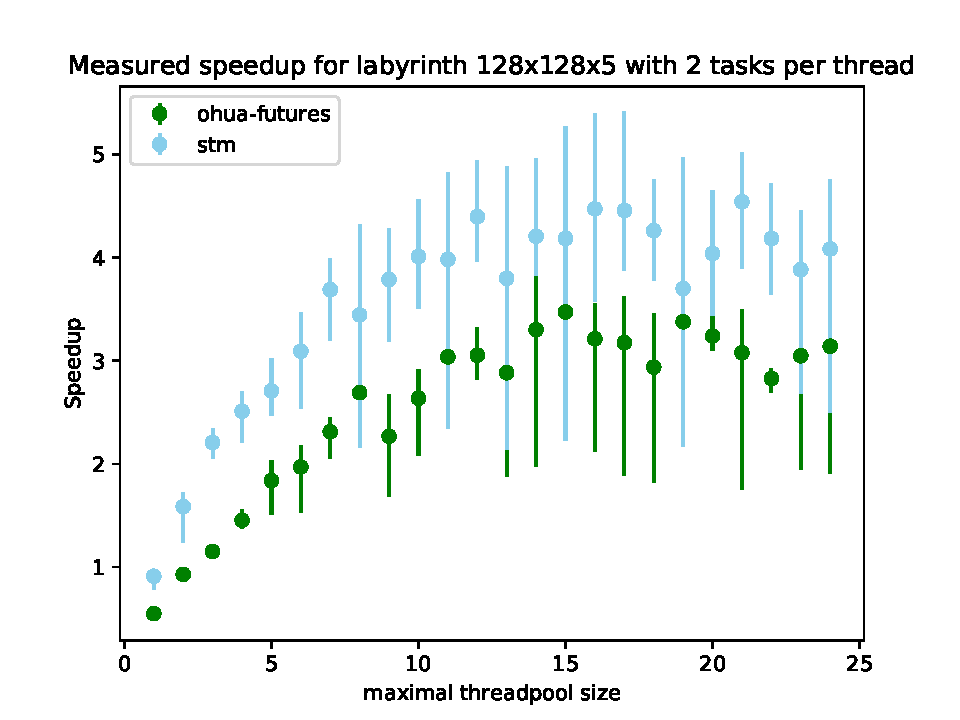
\includegraphics[width=.5\textwidth,keepaspectratio]{gfx/preliminaries-labyrinth/current-128x128x5}
    \caption{Measured speedup for an Ohua implementation using worklist splits, an update frequency of $2 \cdot threadcount$ and a work-stealing runtime.}%
    \label{fig:preliminaries:future-results}
\end{figure}

In employing this runtime, we hoped to reduce the slack time seen in our first parallel implementation by moving work away from the longer-running threads to ones that finished quicker.
Figure~\ref{fig:preliminaries:future-results} confirms this.
Ohua now manages to achieve a threefold speedup compared to a sequential implementation of the benchmark, closing in on STMs performance.
It also benefits from its deterministic execution model, exhibiting a lower variation in the measured values than STM.\todo{calculate standard deviation?}
The higher variance in STMs results is mainly due to the non-deterministic execution model, leading to a varying commit order for the mapped paths with each execution.
This influences, which paths can be mapped successfully in a single run and how many write conflicts occur during execution which in turn has a direct effect on the predictability of the execution time.
Ohua on the other hand is more deterministic.
All paths are mapped in parallel, but they are merged in the same order they were in before being processed, yielding reproducible results that can be easily debugged and do not underlie a similarly high deviation.
Due to the scattering of STMs results, one can not with definitive certainty say whether it indeed outperforms Ohua for every thread count value as the variances sometimes overlap, e.g., for 11, 13 and 15 threads.

All in all, these preliminary studies showed that in irregular applications, Ohua can achieve performances similar to Software Transactional Memory if the right transformations are applied to the algorithm.
This warrants further investigation by trying to find generalized dataflow graph transformations which can be applied to Ohua algorithms in order to boost their performance at runtime.


% !TEX root = ../thesis.tex
%
\chapter{Compiler Transformations}
\label{sec:transformations}

After discussing possible optimizations to the labyrinth algorithm in Chapter~\ref{sec:preliminary}, we will now attempt to generalize the changes we made into transformations to be applied at compile time.
The resulting transformations will be formally described and their correctness discussed in this chapter, using an Expression IR that is based on the lambda calculus.
An implementation of the presented transformations will be left for future work.

\section{Expression IR Definition}%
\label{sec:transformations:expression-ir}

\begin{figure}[p]
    \begin{tabular}{l c l r}
        \multicolumn{4}{l}{\emph{Terms:}}\\
        $t$ & $::=$ & $x$ & variable\\
        & $|$ & $\lambda x.t$ & abstraction\\
        & $|$ & $t\ t$ & application\\
        & $|$ & \texttt{let} $x = t$ \texttt{in} $t$ & lexical scope (variable binding)\\
        & $|$ & \texttt{if}$(t\ t\ t)$ & conditionals\\
        & $|$ & \texttt{let} $f = \lambda x.t$ \texttt{in} $t$ & fixed-point combinator\\
        & $|$ & $\texttt{ff}_f (x_1 \dots x_n)$ & apply the free foreign function $f$ to $x_1 \dots x_n$\\
        &&& with $n \geq 0$.\\
        & $|$ & $\texttt{sf}_f (s\ x_1 \dots x_n)$ & apply the state-modifying foreign function $f$\\
        &&& to state $s$ and $x_1 \dots x_n$ with $n \geq 0$.\\\ \\
    
        \multicolumn{4}{l}{\emph{Values:}}\\
        $v$ & $::=$ & $o \in V_\text{h}$ & value in host language\\
        & $|$ & $\lambda x.t$ & abstraction\\
        & $|$ & $[ v_1 \dots v_n ]$ & list of $n$ values\\\ \\ \
    \end{tabular}
    
    \begin{tabular}{l c l}
        \multicolumn{3}{l}{\emph{Predefined Functions:}}\\
        \texttt{map}$(\lambda x.t\ [ v_1 \dots v_n ])$ & $\equiv$ & $[ (\lambda x.t)\ v_1\ \dots \ (\lambda x.t)\ v_n ]$\\
                                                       && given that $\texttt{sf}_f \notin t$\\
                                                       &&\\
        \multirow{4}{*}{\texttt{map}$(\lambda s_0\ x.t\ [ v_1 \dots v_n ])$} & \multirow{4}{*}{$\equiv$} & $\texttt{let } s_1\ y_1 = (\lambda s_0\ x.t)\ v_1 \texttt{ in}$\\
                                                            && \hspace*{.3cm}$\dots$\\
                                                            && \hspace*{.6cm}$\texttt{let } s_n\ y_n = (\lambda s_{n-1}\ x.t)\ v_n \texttt{ in}$\\
                                                            && \hspace*{.9cm}$ [s_n\ [y_1 \dots y_n]]$\\
                                                            && given that $\texttt{sf}_f  \in t$\\
                                                            &&\\
        \texttt{nth}$(n \ [ v_1 \dots v_n \dots v_p])$ & $\equiv$ & $v_n$\\
        \texttt{split}$(n \ [ v_1 \dots v_p])$ & $\equiv$ & $[ [v_1 \dots v_{\frac{p}{n}}]\ \dots \ [v_{\frac{(n-1) p}{n} + 1} \dots v_p] ]$\\
        \texttt{join}$([ [v_1 \dots v_{\frac{p}{n}}]\ \dots \ [v_{\frac{(n-1) p}{n} + 1} \dots v_p] ])$ & $\equiv$ & $[ v_1 \dots v_p]$\\
        \texttt{take\_n}$(n \ [ v_1 \dots v_n \dots v_p])$ & $\equiv$ & $[ [v_1 \dots v_n]\ [v_{n + 1} \dots v_p] ]$\\
        \texttt{len}$([ v_1 \dots v_n ])$ & $\equiv$ & $n$
    \end{tabular}
    \caption{Language definition of the Expression IR.}%
    \label{fig:transformations:definition}
\end{figure}

\begin{figure}[p]
    $\texttt{let } f = \lambda x_{\text{maze}}\ x_{\text{points}}.$\\
    \hspace*{.3cm}$\texttt{let } f_\text{body} = \lambda y\ z.$\\
    \hspace*{.6cm}$\texttt{let } x_\text{path} = \texttt{ff}_\text{find\_path} (y\ z) \texttt{ in}$\\
    \hspace*{.9cm}$\texttt{sf}_\text{update}(y\ x_\text{path}) \texttt{ in}$\\
    \hspace*{.6cm}$\texttt{let } x_\text{resulting\_maze}\ x_\text{map\_results} = \texttt{map} (f_\text{body}\ x_\text{maze}\ x_\text{points}) \texttt{ in}$\\
    \hspace*{.9cm}$\texttt{let } x_\text{unmapped} = \texttt{ff}_\text{get\_unmapped} (x_\text{map\_results}) \texttt{ in}$\\
    \hspace*{1.2cm}$\texttt{if } ( \texttt{ff}_\text{count} x_\text{unmapped} = 0$\\
    \hspace*{2cm}$x_\text{resulting\_maze}$\\
    \hspace*{2cm}$f\ x_\text{resulting\_maze}\ x_\text{not\_mapped}) \texttt{ in}$\\
    \caption{Expression for our labyrinth algorithm.}%
    \label{fig:transformations:ir-first-stage}
\end{figure}

During compilation, the Ohua compiler framework parses algorithms provided as inputs into an Expression IR on which it then runs a number of optimizations~\cite{ertel2018compiling}, as we have shown in Figure~\ref{fig:background:ohua} in Chapter~\ref{sec:background:ohua}.
We are going to describe our transformations in this intermediate representation, which we will therefore present now briefly.
The Expression IR we use is based on the call-by-need lambda calculus~\cite{ariola1997lambda, ariola1995lambda} which prevents duplicated computations.
Figure~\ref{fig:transformations:definition} defines our expression language, which is building atop the language used in previous research on Ohua optimizations~\cite{ertel2018compiling} by Ertel et al.
The language defines the basic terms of the call-by-need lambda calculus for variables, abstractions, application and lexical scoping.
We additionally define conditionals and fixed-point combinators to realize recursive expressions as well as free and state-modifying foreign functions.
Using the combinator $\text{ff}_f$, one can express the application of a function $f$ which is not defined as part of the calculus to an arbitrary number of arguments.
This allows us to integrate code written in other languages like Rust into the algorithm, which is a key premise for Ohua's concept as Embedded DSL.
Furthermore, we expand the definitions used in previous work by adding the combinator $\text{sf}_f$, which applies a method $f$ to a state value $s$ and an arbitrary number of additional values.
We made this addition in order to model the state manipulations usually found in shared state applications.
Methods that are executed on a state value may alter it but are usually also allowed to return another value (e.g., when reading from a piece of state).
This behavior is reflected in the \texttt{sf} combinator producing a list with two values as result, where the first value is the the altered state value and the second value is the ordinary value produced by the function $f$.

In order to complete the inclusion of legacy code into the Expression IR, values may not only be abstractions or lists of values but also values in $V_\text{h}$, the value domain of the host language.
Aside from recursion, we also define the well-known higher-order function \texttt{nth} to retrieve a particular element from a list of values.
The function \texttt{map} applies a term to a list of values.
Depending on whether the term applied contains a stateful function or not, the definition of the function differs as state updates need to be applied during loop execution.
Both the definition of the \texttt{sf} combinator and the handling of it inside a map operation are based on the notion of state threads which were introduced to Ohua by Ertel et al. in recent work~\cite{ertel2019stclang}.
The function \texttt{split} separates an input list into equally sized chunks, while the function \texttt{join} reverses this operation, flattening a list of lists into a single large list.
Both functions cancel each other out:
\begin{align*}
    \texttt{join}(\texttt{split}(n \ [v_1 \dots v_p])) \equiv [v_1 \dots v_p]
\end{align*}
The function \texttt{take\_n} splits the input list into two parts, where the first list contains the first $n$ elements (or the whole input list, whichever is smaller) and the second list forms the remainder of the input list.
\texttt{len} is a simple function to determine the length of a list.

As a shorthand for writing more concise terms, we introduce a simple destructuring syntax which has already been used in the definition of \texttt{map} and is defined as follows:
\begin{center}
    \begin{tabular}{l c l}
        && \texttt{let} $x_{\text{result}} = \texttt{ff}_f() \texttt{ in}$\\
        \texttt{let} $y\ z = \text{ff}_f() \texttt{ in}$ & $\equiv$ & \ \ \texttt{let} $y = \texttt{nth}(1\ x_{\text{res}}) \texttt{ in}$\\
        && \ \ \ \ \texttt{let} $z = \texttt{nth}(2\ x_{\text{res}}) \texttt{ in}$\\
    \end{tabular}
\end{center}

\begin{listing}[!b]
    \begin{minted}{Rust}
        fn fill(maze: Maze, points: Vec<(Point, Point)>) -> Maze {
            let map_results = for pts in points {
                let path = find_path(maze, pts);
                maze.update(path)
            }

            let unmapped = get_unmapped(map_results);
            if unmapped.len() == 0 {
                maze
            } else {
                fill(maze, unmapped)
            }
        }
    \end{minted}
    \caption{Idiomatic definition of the labyrinth algorithm.}%
    \label{fig:transformations:idiomatic}
\end{listing}

Using our defined calculus, we can now define an expression that describes our labyrinth benchmark from Chapter~\ref{sec:preliminary:labyrinth}.
As point of origin, we use an idiomatic declaration of the labyrinth algorithm which is more compact than any version in the aforementioned chapter and resembles the algorithm as it would be written by a developer.
This version is shown in Listing~\ref{fig:transformations:idiomatic}.
Notably, we removed the loop split that allowed us to exploit some initial parallelism in Chapter~\ref{sec:preliminary}.
In the corresponding Lambda Expression in Fig.~\ref{fig:transformations:ir-first-stage} we bind the \texttt{fill} algorithm to a fixed-point combinator $f$.
In it, we bind the body of the loop to $f_\text{body}$, to which we then apply the initial state value $x_\text{maze}$.
The resulting partial binding is then mapped onto the list of input values, namely $x_\text{points}$.

\pagebreak

\section{Transformation 1: Map Parallelization}%
\label{sec:transformations:tf1}

The base idea of our first optimization developed in Chapter~\ref{sec:preliminary:tf1} was to execute the path finding in parallel to make use of the multi-threading functionalities of modern commodity CPUs.
This was possible because the path-finding loop was altered to not contain any state update and the loop iterations themselves were therefore independent of one another.
Since we want to have as few application logic as possible in the code generation and the runtime, it makes sense to move this optimization into the Expression IR optimization stage.
To achieve a low-cost parallelization that does not require any knowledge about parallel loops in the runtime, we simply split the loop in question into a number of smaller loops.
As these small loops do not exhibit any data dependencies between one another, the execution runtime can run them in parallel without having to understand, what these operators are.

Although we did this in our specific example for the problem of pathfinding, this can indeed be generalized.
Each \texttt{map} combinator which does not modify state internally, i.e., does not entail \texttt{sf} combinators, may be parallelized in this way.
Using the predefined functions \texttt{split} and \texttt{join} we define the transformation to adapt a map operation for $p$ threads:

\begin{figure}[h]
    \begin{tabular}{l c l}
        \multirow{5}{*}{$\texttt{let } r = \texttt{map} (t\ [v_1 \dots v_n]) \texttt{ in}$} & \multirow{5}{*}{$\underset{\text{p threads}}{\longrightarrow}$} & $\texttt{let } m_1 \dots m_p = \texttt{split} (p\ [v_1 \dots v_n]) \texttt{ in}$\\
                                                                                            &&\hspace*{.3cm} $\texttt{let } r_1 = \texttt{map} (t\ m_1) \texttt{ in}$\\
                                                                                            &&\hspace*{.6cm} $\dots$\\
                                                                                            &&\hspace*{.9cm} $\texttt{let } r_p = \texttt{map} (t\ m_p) \texttt{ in}$\\
                                                                                            &&\hspace*{1.2cm} $\texttt{let } r = \texttt{join} ([r_1 \dots r_p]) \texttt{ in}$\\
    \end{tabular}
    \caption{Transformation 1: Map Parallelization for $p$ threads.}%
    \label{fig:transformations:tf1}
\end{figure}

This transformation turns a single stateless map operation into $p$ independent map operations which can then be individually scheduled and executed.
To prove the semantic correctness of this transformation, we can show that the left and the right expression are indeed equivalent by resolving the right expression bottom-up:
\begin{align*}
    \texttt{join} ([r_1 \dots r_p]) &\equiv \texttt{join} ([\texttt{map} (t\ m_1) \dots \texttt{map} (t\ m_p)])\\
                                    &\equiv \texttt{join} ([[t\ v_1 \dots t\ v_{\frac{p}{n}}] \dots [t\ v_{\frac{(n-1) p}{n} + 1} \dots t\ v_p]])& \text{\small by map definition}\\
                                    &\equiv \texttt{join} (\texttt{split} (p\ [t\ v_1 \dots t\ v_n]))\\
                                    &\equiv [t\ v_1 \dots t\ v_n]\\
                                    &\equiv \texttt{map} (t\ [v_1 \dots v_n])
\end{align*}

Using this rather simple transformation we are now able to split state-free loops into smaller chunks of work that can be executed in parallel due to the absence of data dependencies.

\section{Transformation 2: State Decoupling}%
\label{sec:transformations:tf15}

In its initial state, a loop containing a state update, i.e., a \texttt{smap}, cannot be executed in parallel as the state update must occur sequentially to avoid locking and guarantee a deterministic execution.
In our labyrinth example, we circumvented this by splitting the state update off and running it after the parallel path search from the start.
But to allow any parallelization and later transformations to occur in unaltered applications like the algorithm in Listing~\ref{fig:transformations:idiomatic}, the state-free parts of such a loop must be decoupled from the state update first, using a transaction which we will define and discuss in this intermediate step first.

To formalize this, we let $t$ be a non-empty term that does not contain any state-modifying foreign functions.
We require non-emptiness here because otherwise the \texttt{map} function would only contain a \texttt{sf} combinator in which case no parallelization can occur.
Furthermore, we define a state-modifying foreign function $\texttt{sf}_f$ and values $v_1 \dots v_n$ which are argument to \texttt{sf} and are bound either by the lambda expression mapped over of within $t$.
The initial state value $s$ is bound outside the \texttt{map} combinator.
We can now define this preliminary transformation as follows:
\begin{center}
    \begin{tabular}{l c l}
        & \multirow{7}{*}{$\longrightarrow$} & $\texttt{let } x_\text{intermediate} = \texttt{map} ((\lambda s\ x.t\ [v_1 \dots v_n])$\\
        $\texttt{map} ((\lambda s\ x.t$ && \hspace*{4cm}$[x_1 \dots x_n]) \texttt{ in}$\\
        \hspace*{1.65cm}$\texttt{sf}_f (s\ v_1 \dots v_n))$ && \hspace*{.3cm}$\texttt{map}(( \lambda s\ y. \texttt{let } v_1 \dots v_n = y \texttt{ in}$\\
        \hspace*{.9cm}$[x_1 \dots x_n])$ && \hspace*{2.25cm}$\texttt{sf}_f (s\ v_1 \dots v_n))\ s$\\
                                          && \hspace*{1.1cm}$x_\text{intermediate})$
    \end{tabular}
\end{center}

This transformation splits the \texttt{sf} combinator off from the rest of the loop body, allowing the first to be parallelized using Transformation 1 from Section~\ref{sec:transformations:tf1}.
It represents a frequent pattern in shared state scenarios, where such loops often act as a fold operation on the state value.

But while this transformation enables us to further optimize state loops, we also have to discuss whether this is a legitimate optimization to make or whether it may alter the semantics of the program in question.
For the previous transformation, showing the equivalence of both terms was simple and could therefore be done.
For this alteration however, this would unwind into a lengthy proof which would be out of scope for this thesis and shall therefore be left for future work.
Moreover, one can see easily, that an expression can be constructed that, given the same input, will not produce the same results before and after the transformation.
An example that immediately comes to mind is the labyrinth algorithm.
When searching a path, the \texttt{find\_path} function reads the current state value which will ater the application of the transformation at no point contain any of the previously found paths.
This produces numerous write conflicts, forcing recomputations and generating commits in a different order than in the sequential version, eventually leading to different results.
% Even though equivalence may be shown for many expressions which do not read state to produce the value for the update\footnote{An example are producers in a classical producer-consumer scheme where the buffer between both is filled using a state update.}, one generally has to assume that this criteria does not hold.
However, this is also the case for other parallelism approaches like \emph{Software Transactional Memory}, which also does not preserve equivalence to a sequential execution.
This is due to the amorphous data parallelism often encountered in these shared state programs.
There is just no way to efficiently parallelize these applications without encountering their side effects and in particular while retaining sequential equivalence.
Hence, we argue that this transformation is nonetheless valid, especially when migrating the application from a STM background.
What's more, this approach manages to retain one of the core promises of Ohua: Determinism.
Even though the results from before and after applying the transformation are not equivalent, they are both deterministic, which cannot be said about STM whose model is founded on non-deterministic execution.
On the other hand, when attempting to parallelize such an application for the first time, developers should be well aware of the fact that parallelizing amorphous data parallel programs comes with trade-offs, making our approach still seem a good fit.

\section{Transformation 3: Batch Updates}%
\label{sec:transformations:tf2}

The second optimization we put forth in Chapter~\ref{sec:preliminaries:retries} considered itself with improving execution times by batching state updates.
Our general idea was that the state update forms a sequential bottleneck which severely decreases performance.
After the application of the transformation described in Section~\ref{sec:transformations:tf15} however, we found that the isolated state updates gave way to the negative side effects of applications exhibiting amorphous data parallelism which mainly manifested in increased write conflicts due to infrequent updates.
Hence, we wanted to introduce a way to vary the frequency of state updates in order to have a way to reduce the number of conflicts.

In our preliminary studies, we tackled this problem by only ever processing an arbitrary but fixed number of elements before updating the state.
Although we mixed the retry semantics of the algorithm itself with the update frequency approach in Chapter~\ref{sec:preliminaries:retries} by immediately appending any failed updates to the back of the work set instead of putting them in a separate list, we can distill a generic transformation from this approach.
Basic idea for this transformation is to turn the stateful loop into a recursive combinator that always takes up to $n$ elements per recursion step from the input set and processes them until all elements have been processed.
To formalize this we let $n$ be the number of items to be processed per step.
As for the previous transformation, $s$ defines the initial state value and is bound outside of the \texttt{map} expression, while $[x_1 \dots x_p]$ is the set of input values for the map operation.
The term $t$ does not contain any \texttt{sf} combinators and the values $v_1 \dots v_p$ are all bound within the scope of the lambda expression mapped over.
The transformation is then defined as follows:
\begin{center}
    \begin{tabular}{l}
        $\texttt{map} ((\lambda s\ y.t\ \texttt{sf}_f(s\ v_1 \dots v_p))\ s\ [x_1 \dots x_p])$\\
    \end{tabular}

    $\downarrow$

    \begin{tabular}{l}
        $\texttt{let } r = \lambda s_0\ x.$\\
        \hspace*{.3cm}$\texttt{let } x_\text{input}\ x_\text{rest} = \texttt{take\_n}( n\ x) \texttt{ in}$\\
        \hspace*{.6cm}$\texttt{let } s_\text{new}\ x_\text{result} = \texttt{map} ((\lambda s\ y.t\ \texttt{sf}_f(s\ v_1 \dots v_n))\ s_0 \ x_\text{input}) \texttt{ in}$\\
        \hspace*{.9cm}$\texttt{if} (\texttt{len} (x_\text{rest}) = 0$\\
        \hspace*{1.5cm}$[s_\text{new}\ x_\text{result}]$\\
        \hspace*{1.5cm}$(\texttt{let } s_\text{res}\ x_\text{res} = r\ s_\text{new} \ x_\text{rest} \texttt{ in}$\\
        \hspace*{1.8cm}$s_\text{res}\ \texttt{join} (x_\text{result} x_\text{res})) \texttt{ in}$\\
        \hspace*{.3cm}$r \ s \ [x_1 \dots x_p]$
    \end{tabular}
\end{center}

Note that we used in this transformation a non-decoupled stateful loop for the sake of brevity only.
Transformation 2 may be applied either before or after this step to expose the necessary loop parallelism that warrants this transformation in the first place.

One can see easily, that this transformation also retains Ohua's determinstic approach: All elements are processed in the same order and state updates are also applied in the same, fixed order for each value for $n$.
But, as was the case for Transformation 2 in Section~\ref{sec:transformations:tf15} and has been exhaustively discussed there, semantic equivalence is not preserved by this operation either but is admissible as this is due to the basic properties of amorphous data parallel programs.

\section{Transformation 4: Straggler Reduction using Work Stealing}%
\label{sec:transformations:tf3}

The third modification we presented in Chapter~\ref{sec:preliminary} was the improving of resource utilization by tackling the straggler problem we discovered after parallelizing state-free map operations.
Underlying cause for the straggler problem was the static assignment of work to specific threads.
Due to the non-uniform nature of most map operations encountered in real-world applications and noise introduced by the operating system itself~\cite{lackorzynski2016decoupled}, static work set assignments can produce wildly varying execution times per thread, as seen in Fig.~\ref{fig:preliminary:straggler}.
Hence, we applied a work-stealing task scheduling runtime to improve performance.

Admittedly, this optimization step is hardly a transformation but a mere engineering solution.
It can be applied by changing the code generated for the set of \texttt{map} combinators produced by Transformation 1 presented in Section~\ref{sec:transformations:tf1}.
Instead of generating a number of loop operators as originally intended, we can instead create a work-stealing runtime and schedule the loop operations as tasks in the runtime.

% !TEX root = ../thesis.tex
%
\chapter{Experimental Setup}%
\label{sec:experiments}

In order to compare the performance of Software Transactional Memory against Ohua in the context of shared state applications, we employ a set of benchmarks originally proposed by Minh et al.~\cite{minh2008stamp}.
In this chapter, we will categorize the benchmarks introduced by the authors and present a representative selection of applications which we will use to compare Ohua's performance against STM.
Additionally, we will explain, which values we measured during execution of the benchmarks and how they are relevant for our evaluation.

\section{Benchmark Choice}
\label{sec:experiments:choice}

After presenting our transformations for Ohua in Chapter~\ref{sec:transformations}, we now wanted to compare its performance against STM in order to evaluate if Ohua could indeed be used as a suitable replacement for developing shared state applications.
To provide a comprehensive comparison, we chose to use the \emph{Stanford Transactional Applications for Multi-Processing} suite~\cite{minh2008stamp}.
Introduced by Minh et al., it was designed as a set of benchmarks for testing software transactional memory frameworks.
The authors included 8 applications from different application areas in their suite, which are supposed to resemble the diverse landscape of parallelism in applications developers might face.
In particular, the STAMP suite contains examples from different application domains and varying use cases for transactional memory such as high-contention and low-contention scenarios.

\begin{table}
    \centering
    \begin{tabular}{|l|l|l|}
        \hline
        \textbf{Application} & \textbf{Instructions per tx} \emph{(mean)} & \textbf{Time spent in transactions}\\\hline\hline
        labyrinth & 219,571 & 100\%\\\hline
        bayes & 60,584 & 83\%\\\hline
        yada & 9,795 & 100\%\\\hline
        vacation & 3,223 & 86\%\\\hline
        genome & 1,717 & 97\%\\\hline
        intruder & 330 & 33\%\\\hline
        kmeans & 117 & 7\%\\\hline
        ssca2 & 50 & 17\%\\\hline
    \end{tabular}
    \caption{A basic characterization of STAMP applications, comparing the mean number of instructions per transaction and the overall percentage of time the application spends in transactions. These numbers stem from a C implementation and have been adapted from Minh et al.~\cite{minh2008stamp}}
    \label{tab:experiments:overview}
\end{table}

The tables~\ref{tab:experiments:overview} and~\ref{tab:experiments:categorization} give a basic characterization of the benchmarks in terms of their usage of transactions.
As can be seen in table~\ref{tab:experiments:overview}, the length of individual transactions varies greatly per application, as does the overall time that is spent by the benchmark executing transactions.
Even though the numbers in the table have been adapted from Minh et al.\ and represent values measured for their C-based implementation, they still outline the general characteristics of the respective STM-based algorithms.
Some applications suffer so badly from the irregular properties outlined in Chapter~\ref{sec:background:irregular} that exploiting their parallelism requires them to spend more than 80 \% of their overall execution time in transactions.
This is for example the case in the \emph{labyrinth} benchmark, where fields of a dense 3-dimensional matrix have to be continuously updated, as we explained in Chapter~\ref{sec:preliminary:labyrinth}.
Other applications such as \emph{kmeans} or \emph{ssca2} have relatively short transactions, meaning their data parallelism is easier to exploit or they generally do not feature as much opportunities for parallelism as other applications.

\begin{table}
    \centering
    \begin{tabular}{|l|l|l|l|l|}
        \hline
        \textbf{Application} & \textbf{tx length} & \textbf{r/w set} & \textbf{tx time} & \textbf{Contention}\\\hline\hline
        labyrinth & long & large & high & high\\\hline
        bayes & long & large & high & high\\\hline
        yada & long & large & high & medium\\\hline
        vacation & medium & medium & high & low/medium\\\hline
        genome & medium & medium & high & low\\\hline
        intruder & short & medium & medium & high\\\hline
        kmeans & short & small & low & low\\\hline
        ssca2 & short & small & low & low\\\hline
    \end{tabular}
    \caption{A qualitative summary of each STAMP application's runtime transactional characteristics. The length of a transaction is determined by the number of instructions it encompasses. The characteristics are ranked relative to the other applications in the suite. Adapted from Minh et al.~\cite{minh2008stamp}}
    \label{tab:experiments:categorization}
\end{table}

Another relevant and perhaps the most limiting factor for programs relying on optimistic parallelism principles such as STM is contention.
This characteristic is visualized in table~\ref{tab:experiments:categorization} along with other properties.
When facing high contention scenarios, STM implementations are usually unable to achieve the near-linear speedups Minh et al.\ reported for other benchmarks.
Contention is a byproduct of frequent reading and writing accesses to the shared data structure that inevitably lead to frequent conflicts which require a rollback of all affected transactions except for the one that committed its changes first.
Hence, the relative amount of reads and writes per transaction is also reported in table~\ref{tab:experiments:categorization}.
Long transactions, large read/write sets, more time spent in transactions and high contention are all factors promoting conflicts.
The results of conflicts are frequent rollbacks and accompanying recomputations, which reduce the overall performance.

Based on the analysis provided by the authors, we selected a representative range of benchmarks for our comparison between Ohua and STM.
We chose applications with varying transaction lengths and frequency of transaction use as well as different levels of contention.
The next sections will briefly outline the details of the chosen benchmarks and explain, how they were implemented.


% THEN elaborate further about the technical details that hold true for all benchmarks
Since the authors only provided a C-based reference implementation for their programs, we had to re-implement them in Rust to rule out language-specific performance changes when comparing to Ohua's Rust implementation.
We chose to use the \texttt{rust-stm} library written by Bergmann et al.~\cite{bergmann2020stm} for these implementations.
Upon inspecting the original source code, it turned out that the authors adapted the code in order to improve the performance of STM in some benchmarks.
For instance, they provided their own implementation of a \rust{HashMap}\footnote{A dynamic key-value store allowing fast lookups by hashing the keys and organizing them in different buckets.} that offered the use of transactions on a per-bucket basis, effectively exposing fine-granular parallelization opportunities that normal HashMaps cannot provide.
In Rust, no corresponding STM-specific data structures existed prior to this work.
We debated, whether or not we should use these optimizations in our own implementation but ultimately decided in favor of doing so.
First, one could argue that these optimizations would be made by developers anyway after deciding to use the STM framework in an attempt to tailor the program code towards the library used.
Secondly, we wanted to remain as close as possible to the original implementations from Minh et al.\ in the hopes of achieving similar results for STM as they did.
Therefore, we contributed a small library~\cite{wittwer2020stmdata} which provides data structures like HashMaps and HashSets augmented for the use with transactions.
Both the library and the benchmarks were implemented from scratch based on the descriptions provided by the authors, literature they cited and the code they supplied.
We did so in an idiomatic way, applying both concepts to the problems using the tools the frameworks and the STM data structure library provide natively.
As implementing the Ohua transformations proposed in Chapter~\ref{sec:transformations} has been left for future work, we applied these transformations manually to the algorithms.
The code for all benchmarks we wrote for this thesis may be found online~\cite{wittwer2020benchmarks}.

When implementing the \emph{labyrinth} benchmark, we found that two transactions may deadlock.
We have reported this issue~\cite{wittwer2020stmissue} and resorted to forking and patching the library~\cite{wittwer2020stm} in question to move on with our tests.

%TODO:
%- explain why i chose bench xy
%- explain benches
%  - detail for labyrinth (etc) why they are so hard to parallelise

\subsection{Labyrinth Path Mapping}
\label{sec:experiments:labyrinth}

The labyrinth benchmark we presented in Chapter~\ref{sec:preliminary:labyrinth} based on the work of Swalens et al.~\cite{swalens2016transactional} was originally proposed by Minh et al. as possible benchmark for Software Transactional Memory.
Since we have already analyzed and implemented this application, it was apparent for us to adduce it for our concluding comparison.
Additionally, it is one of very few benchmarks in the suite exhibiting amorphous data parallelism, a trait the authors did not consider when compiling their benchmark list but which they happened to include by coincidence, as it is frequently encountered in real-life applications using shared state, the main use case for transactional memory applications.
Another interesting property of the benchmark was its frequent use of transactions (the whole algorithm is executed within transactions) and the high contention on the shared data structure, which puts the synchronization primitives under heavy stress, as described before.


%The \emph{labyrinth} benchmark implements a variation of Lee's algorithm \cite{lee1961algorithm} which was conceived to solve path-connection problems that often arise e.g., when searching for an optimal route or when constructing wiring diagrams in electrical engineering.
%Watson et al.~\cite{watson2007study} were the first to implement the algorithm using transactional memory techniques to measure the performance on such systems.
%Based of their algorithm description, we implemented the benchmark, as it has been described in Chapter~\ref{sec:preliminary}\todo{verify correctness of this link}.
%\todo{complete this: Ohua-Impl -> was ist parallel?, original perf \& expected perf}

\subsection{Intruder Detection}
\label{sec:experiments:intruder}

The intruder application implements a signature-based Network Intrusion Detection System (NIDS) and is used in networking to detect attacks or malicious activities in an active network as well as policy violations.
It is based on design proposal number five of Haagdorens et al.'s work on \enquote{Improving the Performance of Signature-Based Network Intrusion Detection Sensors by Multi-Threading}~\cite{haagdorens2004improving}.

The basic function of this application is to scan incoming network packets and match them against known intrusion signatures.
This happens in three distinct stages, as outlined in Fig.~\ref{fig:experiments:intruder:workflow}.
Incoming network traffic is captured and queued for inspection.
Due to the architecture of modern network protocols, individual data flows have to be split into several packets that are transmitted individually and may reach the recipient out of order.
Attackers have used this in the past by splitting malicious flows and sending them out of order to avoid detection.
To counter this, the second step in the algorithm is to deploy stateful detection avoidance countermeasures, which involve preprocessing the received packets and reassembling the original flows.
These flows can then finally be matched against known attack patterns, filtering any malicious packets from the stream of incoming data.

\begin{figure}
    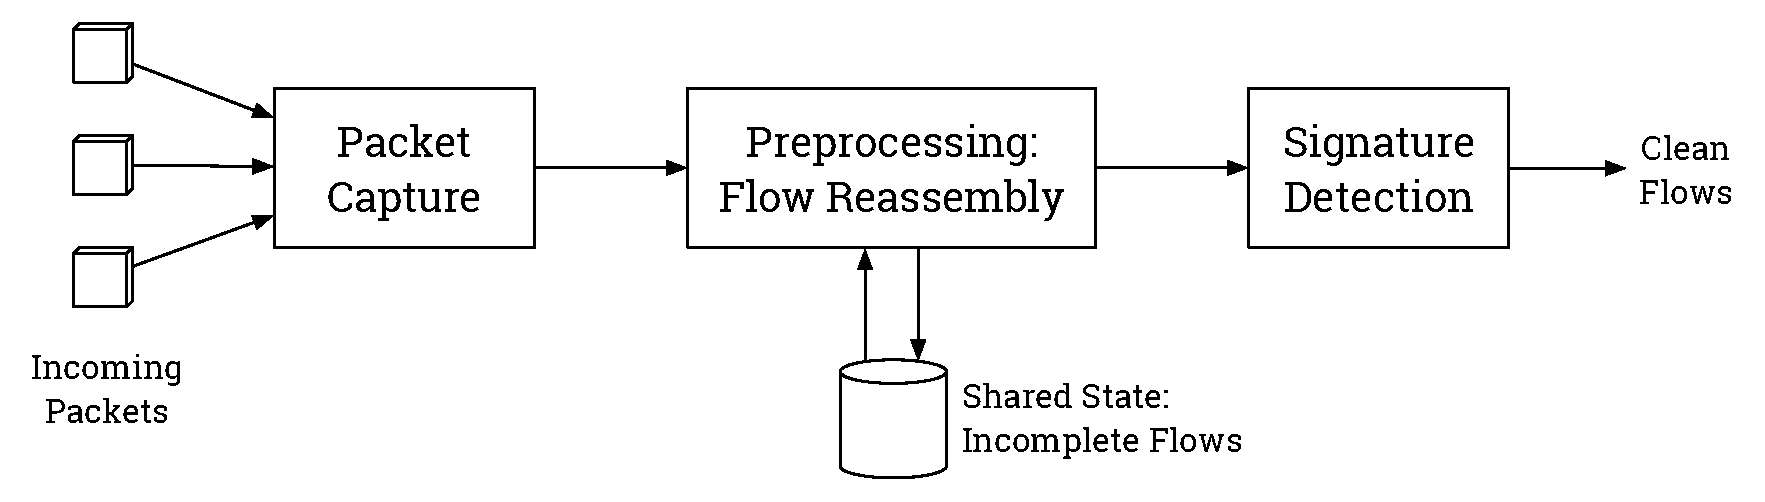
\includegraphics[width=\textwidth,keepaspectratio]{gfx/experiments-intruder}
    \caption{Workflow of the \emph{intruder} benchmark. Processing of incoming data is conducted in three stages.}%
    \label{fig:experiments:intruder:workflow}
\end{figure}

While our STM implementation performs the steps two and three in parallel, in Ohua only the third step is parallelized by the compiler since the second step consists only of a loop that writes all inputs to a state value.
Since the loop body does not contain any other state-free functions, there are no parallelization opportunities for Ohua as no transformations from Chapter~\ref{sec:transformations} are applicable.
Step three however consists of a state-free loop where all inputs are checked for malicious data flows, something that can easily be optimized by applying Transformation 1 as presented in Chapter~\ref{sec:transformations:tf1}.
This shows that Ohua may only extract parallelism from irregular applications that fit certain criteria, i.e., contain loops that do not solely consist of state-modifying operations, as its main approach is to exploit data parallelism by the use of certain transformations to uncover it.

This benchmark was chosen because it is mostly similar in its properties to the labyrinth application as it also features short transactions and high contention on the shared data, but does only spend about 33 \% of the overall execution time in transactions.
We mainly wanted to see, how this slight difference in properties is reflected in the performance results.


\subsection{K-means Clustering}
\label{sec:experiments:kmeans}

Proposed as benchmark by Narayanan et al.~\cite{narayanan2006minebench} the k-means clustering algorithm partitions a set of $n$ observations into $k$ clusters.
It was originally put forth by MacQueen et al. in 1967~\cite{macqueen1967some} and still is a very popular algorithm for cluster analysis in data mining which is often used to classify data.

The inner workings of the algorithm are rather simple: It takes a set of $n$ observations and a desired number of clusters to sort the observations into.
Then the $k$ cluster centroids are initialized.
Many ways exist to realize this but we chose, akin to our C reference implementation, to select the coordinates for each cluster centroid randomly from the coordinates preset by the input data set.
Following this initialization, each observation is assigned to its nearest cluster based on the squared multi-dimensional spatial euclidian distance between both points.
Afterwards, new centroids are computed by calculating the means of all observations now assigned to a certain cluster.
These last two steps now get repeated iteratively until the algorithm either reaches an upper bound of iterations or converges, i.e., less than a certain percentage of observations change per iteration.

In the STM version each iteration is executed completely in parallel, splitting the input dataset equally among the executing threads and guarding access to the centroids and the delta value, which is used for deciding on convergence, using transactions.
Ohua also does each iteration in parallel using Transformation 1 and 4 to exploit data parallelism although the loop has been written in the algorithm in a way to make sure no shared state exists within.

k-means is very much like the intruder benchmark in the regard that its parallelism opportunities are limited to a single state-free loop but unlike the aforementioned benchmark k-means features low contention on shared data structures while presenting a similar transaction utilization, making this an interesting benchmark to look at.

\subsection{Genome Sequencing}
\label{sec:experiments:genome}
This benchmark implements a \emph{\enquote{whole-genome shotgun sequencing}} algorithm as outlined by Pop et al.~\cite{pop2002genome} in their work.
Its goal is to sequence a (fictional) genome, i.e.\ to reassemble a nucleotide sequence from a set of snippets which is something frequently done in genetics.

\begin{figure}[b]
    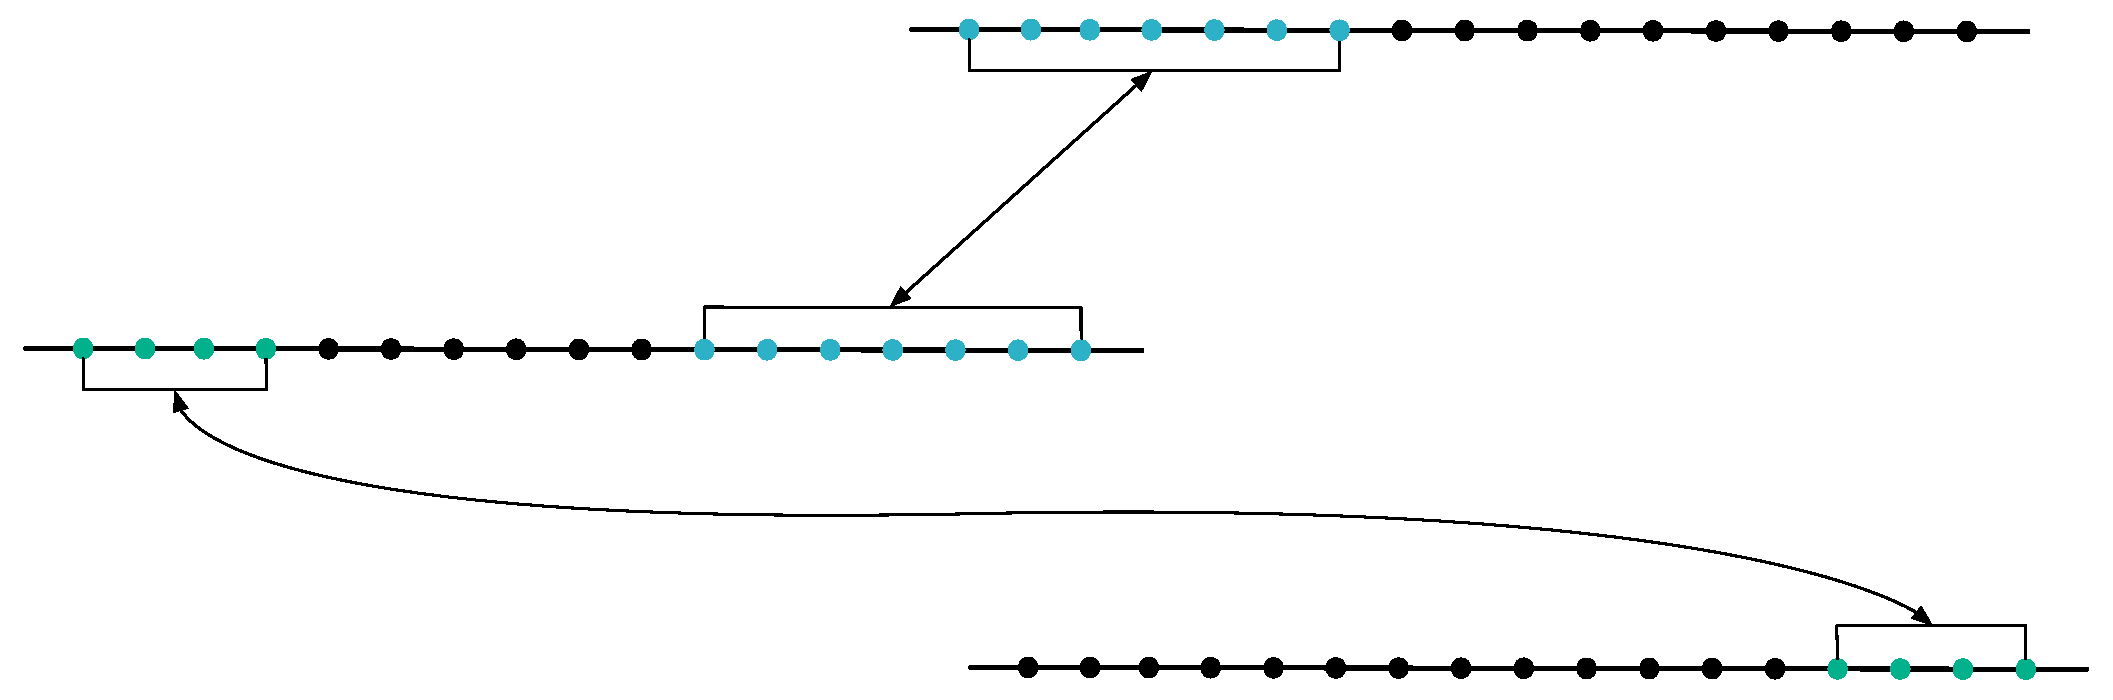
\includegraphics[width=\textwidth,keepaspectratio]{gfx/experiments-genome}
    \caption{Visualization of the overlap matching found in the \emph{genome} benchmark. The blue match is stronger as it has seven matching elements and has hence been found first.}
    \label{fig:experiments:genome-example}
\end{figure}

The first step in the algorithm is to deduplicate the DNA segments that have been provided as inputs, since there are usually many duplications.
The second phase is then concerned with finding neighboring segments in the remaining pool of DNA parts by utilizing overlap matching.
By reducing the overlap size each iteration, the best possible fit is chosen for each neighbor search.
Figure~\ref{fig:experiments:genome-example} provides visualization of how this matching works.
Starting from a match length of $n-1$, the algorithm attempts to find a matching predecessor-successor pair for all loose ends.
With each iteration, the match length is reduced, until it ends with an overlap of one.
In our example, the blue overlap match is found first due to seven matching nucleotides.
Three iterations later, the green match is established, fully connecting the centered genome segment.
After this phase has finished, all but two segments have a predecessor and successor assigned.
Starting from the one element in the set with no predecessor, the chain of nucleotides can be rebuilt by simply following the links.

In our STM implementation, the deduplication phase as well as the matching phase are implemented in parallel using a transaction-aware hash set implementation for the first and a doubly-linked list for the latter.
Although we cannot provide an implementation for a hash set that can be shared using Ohua, we opted to assist the compiler in uncovering parallelism in the deduplication step by manually partitioning the worklist beforehand, so that the compiler may break the resulting state-free loop using the first transformation:
\begin{minted}{Rust}
fn dedup(segments: Segments, threadcount: usize) -> Vec<SequencerItem> {
    let parts = partition(segments, threadcount);
    for p in parts {
        deduplicate(p)
    }
}
\end{minted}
The second step is also a simple state-free loop, which can be easily parallelized by just applying transformation four.
This application example shows, that even when using Ohua, code sometimes has to be written in a certain way to expose the parallelism opportunities of a computation to the compiler.
Nevertheless, the resulting Ohua algorithms can still be executed as a sequential program while the resulting STM code, which is even more optimized by the use of special data structures, is unable to do so.

Overall we chose this application to complete our benchmark selection as it provides similar properties as the kmeans benchmark in terms of transaction length and contention but spends nearly all its execution time in transactions, a stark change compared to the 7 \% of transaction time in kmeans.



% - Part 1: Benchmark Choice
%   - which benchmarks did I choose for my thesis, and why? outline the parameters and reasons for the decision
%   - discuss parameters we used to run the benchmarks
%   - Give short overview over the used benchmarks

\section{Measurements}
\label{sec:experiments:measurements}

In our experiments, we tried to achieve reproducible and plausible results so that we can make an educated comparison between both STM and Ohua.
This section will briefly explain our benchmarking setup to enable others to reproduce our results.

\subsection{Input Data}
\label{sec:experiments:measurements:inputs}

For each STAMP application, Minh et al.~\cite{minh2008stamp} additionally provided three sets of parameters to model small, medium and large workloads.
We adopted these parameters with only minor modifications, as intended by the authors.
A change was made to the parameters of the \emph{genome} benchmark as the input data that was randomly created using the original input parameters proved faulty in our re-implementation.
Also, a unnecessary parameter was removed from the \emph{kmeans} benchmark.

\begin{table}
    \centering
    \tiny
    \begin{tabular}{|l l l|}
        \hline
        \textbf{Application} & \textbf{Arguments} & \textbf{Description}\\\hline\hline
        genome & -g 256 -s 16 -n 16384 & \multirow{3}{*}{\begin{minipage}{.4\textwidth}$n$ gene segments of length $s$ are first sampled from a gene consisting of $g$ nucleotides and then reassembled again.\end{minipage}}\\
        genome+ & -g 510 -s 32 -n 32768 & \\
        genome++ & -g 16384 -s 64 -n 16777216 & \\\hline

        intruder & -a 10 -l 4 -n 2048 -s 1 & \multirow{3}{*}{\begin{minipage}{.4\textwidth}From seed $s$, $n$ traffic flows are generated, $a\%$ of which contain attacks. Each flow consists of up to $l$ packets, which are assembled and inspected by the program.\end{minipage}}\\
        intruder+ & -a 10 -l 16 -n 4096 -s 1 & \\
        intruder++ & -a 10 -l 128 -n 262144 -s 1 & \\\hline

        kmeans-high & -n 15 -t 0.05 -i random-n2048-d16-c16.txt & \multirow{6}{*}{\begin{minipage}{.4\textwidth}The input file $i$ containing $n$ points in $d$ dimensions generated about $c$ centers is loaded and then clustered into $n$ clusters. A convergence threshold of $t$ is used.\end{minipage}}\\
        kmeans-high+ & -n 15 -t 0.05 -i random-n16384-d24-c16.txt & \\
        kmeans-high++ & -n 15 -t 0.00001 -i random-n65536-d32-c16.txt & \\
        kmeans-low & -n 40 -t 0.05 -i random-n2048-d16-c16.txt & \\
        kmeans-low+ & -n 40 -t 0.05 -i random-n16384-d24-c16.txt & \\
        kmeans-low++ & -n 40 -t 0.00001 -i random-n65536-d32-c16.txt & \\\hline

        labyrinth & -i random-x32-y32-z3-n96.txt & \multirow{3}{*}{\begin{minipage}{.4\textwidth}The input file $i$ describes a maze of dimensions $x \times y \times z$ and $n$ paths to map.\end{minipage}}\\
        labyrinth+ & -i random-x48-y48-z3-n64.txt & \\
        labyrinth++ & -i random-x512-y512-z7-n512.txt & \\\hline
    \end{tabular}

    \caption{Input data sets for the benchmarks presented in this thesis. Adapted from Minh et al.~\cite{minh2008stamp} and adjusted to mitigate flaws in the original algorithms.}
    \label{tab:experiments:inputs}
\end{table}

Table~\ref{tab:experiments:inputs} gives a full overview over all parameters we used.
Input sets marked with a + indicate a larger input and an appended ++ marks the largest of the three input sets for a benchmark.
The \emph{kmeans} benchmark inputs are additionally labeled as \emph{high} and \emph{low}, which refers to the relative amount of contention produced by the inputs.

\subsection{Measured Values}
\label{sec:experiments:measurements:values}

For the purpose of our comparison between Ohua and STM, two values are of importance and have hence been measured.
As we are calculating the speedups of both implementations in reference to a sequential implementation, the execution time in milliseconds, i.e., the time it takes the algorithm to complete, is relevant.
Moreover, we were interested in the power consumption of both algorithms.
But since measuring the power consumption of the algorithms would have been to complicated and time-consuming, we opted for measuring the total CPU time used by the programs, as the amount of power used while processing is resulting from the utilization of a PCs individual components.
Since all these programs are performing purely in-memory computations, we figured that measuring the CPU time would be a sufficient approximation to draw some general conclusions regarding the power usage.

For both measured values, the setup phase (parsing input arguments and reading input files) and teardown phase (writing the results to a file) where not included in the measurements.
This was done in order to reduce potential noise from Operating System calls resulting from the I/O operations performed in these stages.
Research has shown in the past that this noise, as well as different contention scenarios can severely impact the measured time values, leading to variations in the measured time values.
To take this into account and produce more realistic results, each measurement has been done 30 times, so that statistical outliers do not carry as much weight.
From the resulting measured values the geometric mean was calculated per data point to compile all measurements into a single data point.

Using the measured execution times in Milliseconds, we calculated the speedup using the following equation:
\[
    S_c = \frac{t_{seq}}{t_f}
\]
where $S_c$ is the speedup of the configuration under investigation, $t_{seq}$ is the mean execution time of the sequential implementation and $t_f$ the mean execution time of the framework in question.

\subsection{Running Configuration}
\label{sec:experiments:measurements:hardware}

All benchmarks conducted for this work were run on an Ubuntu 18.04 server with 128GB RAM and two Intel Xeon E5-2630 v2 processors which have a base frequency of 2.60 GHz and offer combined 12 cores with 24 threads.
At all times, the program under inspection was running exclusively on the machine, meaning that aside from background operating system jobs, no other tasks ran on the system simultaneously.

\section{Reference Measurements}
\label{sec:experiments:reference}

Minh et al.\ proposed their STAMP suite in 2008.
Since then, hardware (e.g., clock speeds of CPUs) as well as compile-time optimizations have evolved significantly, rendering the results provided in their paper outdated.
Hence, we decided to run the benchmarks relevant to our investigation again, on the same hardware and under the same conditions as our Rust benchmarks to have a reference we can compare our STM implementations to.
Although the authors themselves only measured results for the smaller two of their three suggested input sets, we tested all three to have a more comprehensive set of results to compare our STM implementation against.

Upon building and executing the benchmarks with the included \texttt{tl2} STM implementation~\cite{minh2013stampcode}, a number of issues with the STAMP suite became apparent, which we already briefly touched upon in Chapter~\ref{sec:introduction}.
The genome benchmark could not be built from the original source code, due to conflicts caused by compile-time memory allocation patching.
We reported this issue~\cite{wittwer2020stampgenome} and employed a workaround to be able to use the benchmark nonetheless.
Additionally, we found that the implementation of the labyrinth benchmark sometimes does not yield a correct solution, causing the program to crash.\todo{[when time] report these issues on gihtub?}
Similar behavior was found for the intruder application, although we did not investigate this further, instead discarding failed runs in both cases, lowering the effective number of test results slightly below 30.
These issues cement some of the drawbacks of STAMP and STM in general, which we discussed in the beginning of this thesis.

For comparability and in order to provide a more complete performance graph, we intended to run the selected four benchmarks also for 1-24 threads but the suite only supports thread counts which are a power of two, leaving us with 1, 2, 4, 8 and 16 threads as test parameters.
Due to this limited result range, we will only be able to draw vague general comparisons between STAMPs STM and our own STM implementation as the sparse result coverage for higher thread counts leaves us unable to reliably identify trends in the performance of STAMP.


% !TEX root = ../thesis.tex
%
\chapter{Results and Evaluation}
\label{sec:evaluation}

In this section, we will present and interpret the results of our experiments as presented in Chapter~\ref{sec:experiments}.
This involves firstly a brief analysis of the results of the original STAMP benchmark to establish them as a baseline to legitimize or discuss the results of our Rust-based STM implementation of the algorithm as we will use the latter to evaluate Ohua's performance.
Subsequently, we will analyze the results of our Ohua benchmarks in detail to see, whether it could be used as a suiting replacement for STM in terms of performance.


\section{Reference Measurement Results}

\begin{figure}
    \centering
    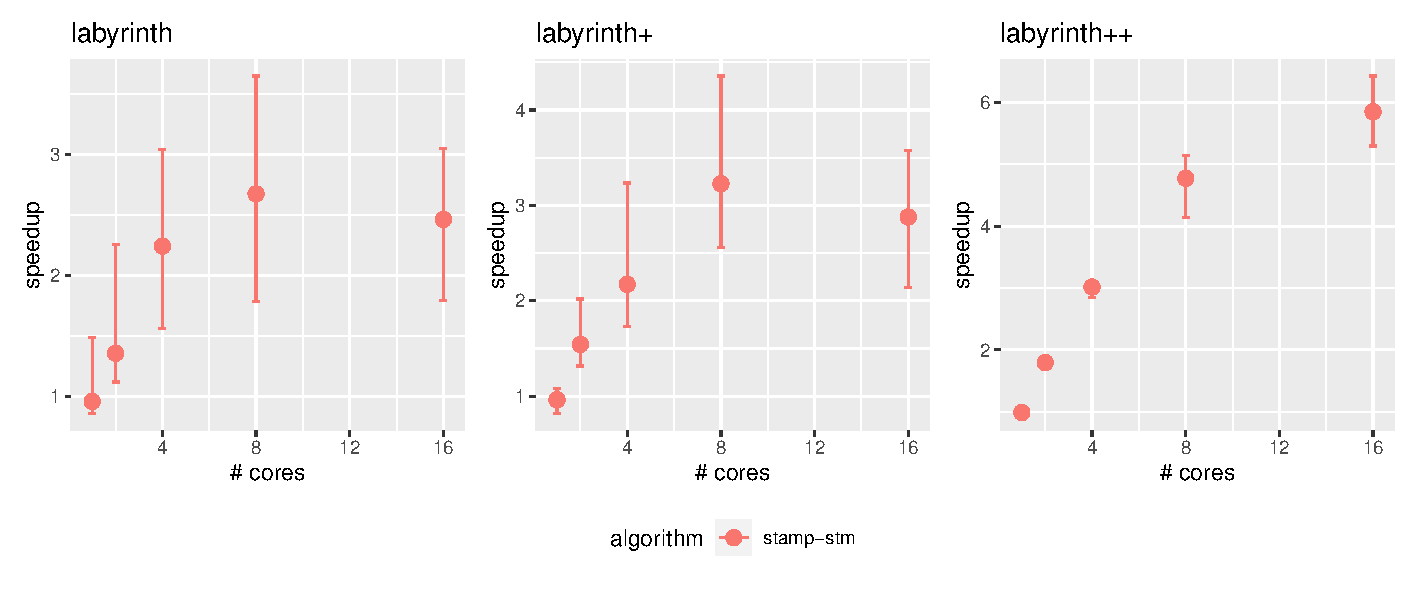
\includegraphics[width=\textwidth,keepaspectratio]{gfx/results/stamp/stamp_labyrinth_comb}
    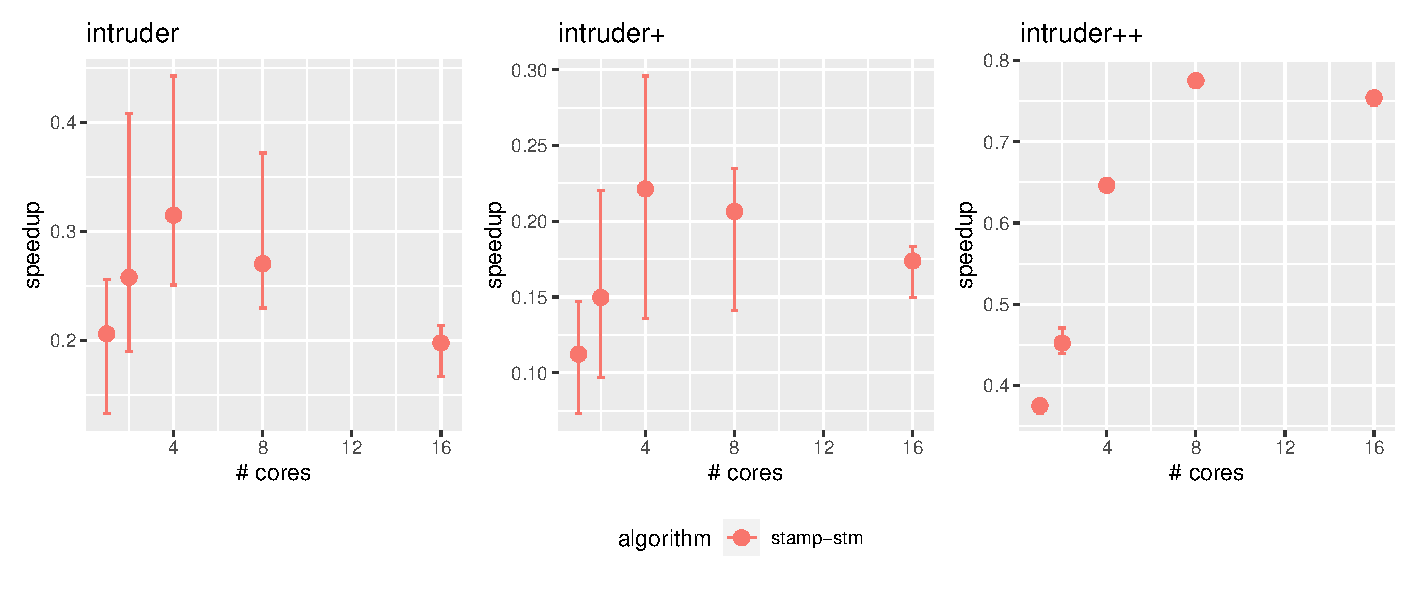
\includegraphics[width=\textwidth,keepaspectratio]{gfx/results/stamp/stamp_intruder_comb}
    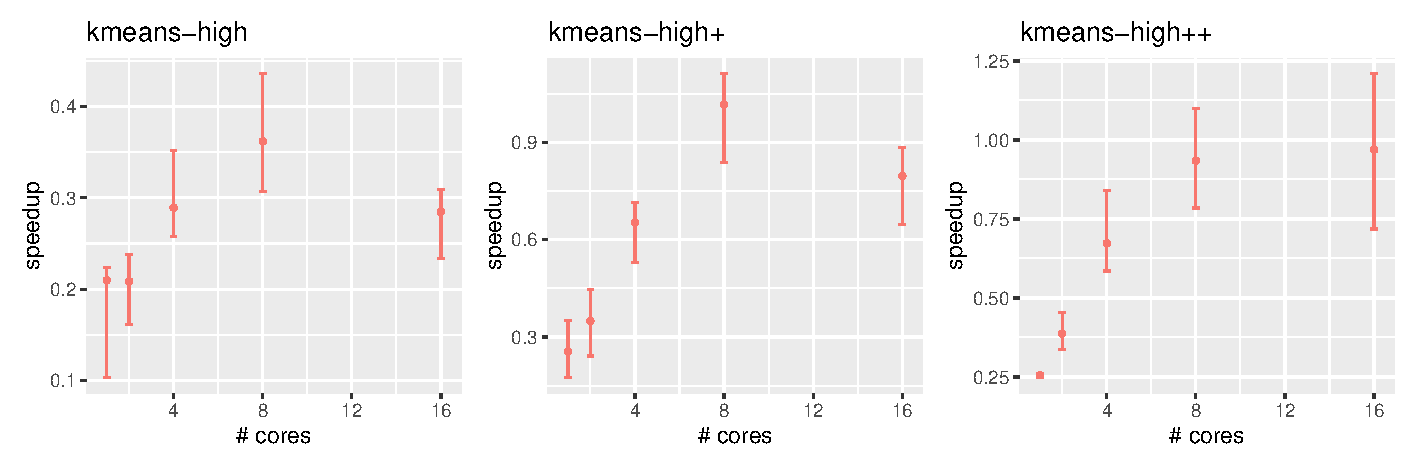
\includegraphics[width=\textwidth,keepaspectratio]{gfx/results/stamp/stamp_kmeans-high_comb}
    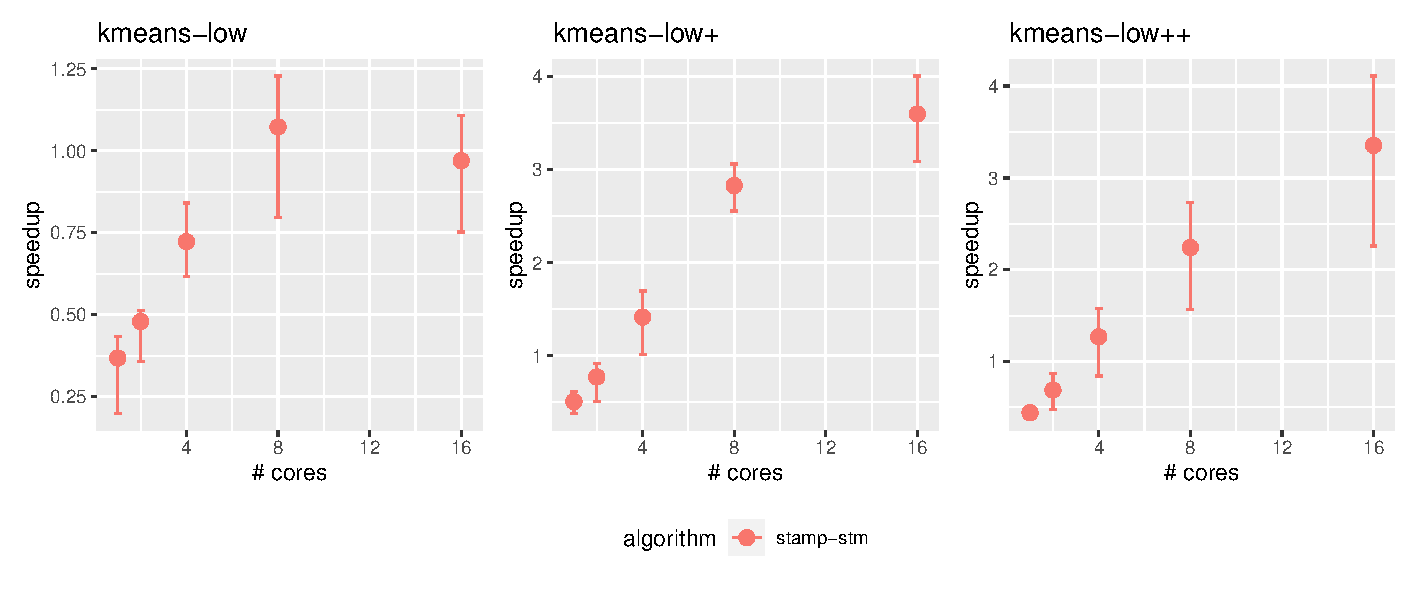
\includegraphics[width=\textwidth,keepaspectratio]{gfx/results/stamp/stamp_kmeans-low_comb}
    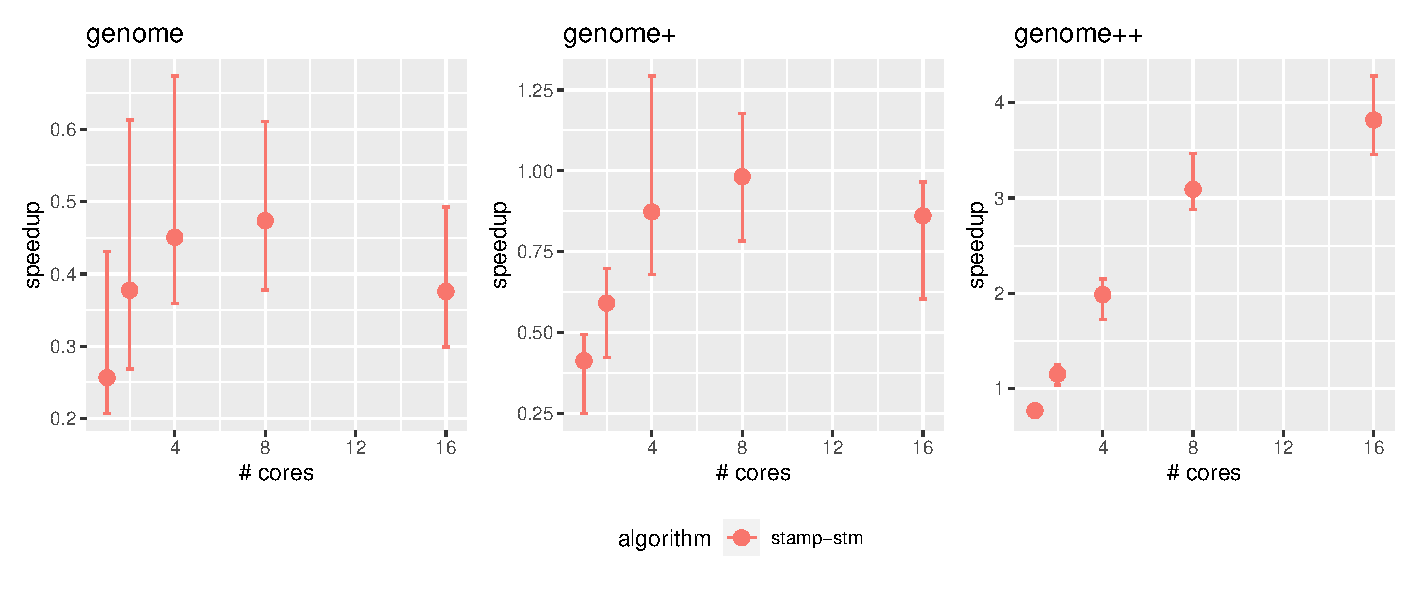
\includegraphics[width=\textwidth,keepaspectratio]{gfx/results/stamp/stamp_genome_comb}
    \caption{Speedup achieved by STM in the original STAMP  benchmarks.}%
    \label{fig:evaluation:stamp}
\end{figure}

Benchmark results for the reference measurement runs we conducted can be found in Figure~\ref{fig:evaluation:stamp}.
We will compare our achieved speedups to the original benchmark runs from Minh et al.~\cite{minh2008stamp}, namely to the results of their Eager STM implementation to see, how performance of the framework changed over the years.
This allows us to set realistic expectations for the performance of our own STM-based benchmark implementations.

In the \emph{labyrinth} benchmark, we observed an increasing speedup for up to 8 threads in the small and medium sized problem sets, maxing at about 3.0 speedup and followed by declining performance for 16 threads.
The largest input data set on the other hand exhibits a steadily increasing curve, achieving a speedup of about 6.0 for 16 threads.
This deviates from the original results, where both the labyrinth and the labyrinth+ benchmark showed behavior similar to our labyrinth++ curve form: A continuously increasing performance, achieving a speedup of about 4.0 at best.
The form of the curve and the overall reduced performance may indicate that either the sequential implementation is performing better now than it did back in 2008 or that the overhead of the \texttt{tl2} STM framework increased.
Our first theory is backed as possible cause by the fact that compiler optimizations have improved in the past years along with CPU clock speeds, making a better sequential performance not unlikely.
An increased framework overhead on the other hand would also support the performance drop for 16 threads, which the better sequential performance does not explain.
Another explanation for this decline would be our used hardware architecture, as it consists of two CPUs.
While all runs up to 8 threads can be executed on a single CPU, the 16 thread version requires the utilization of both cores, requiring more complex memory and resource management which in turn takes more time and may also be an explanation since we do not know if Minh et al.\ had similar hardware.
But since we only made this and the following measurements as reference points for the data we acquired in our own experiments, we did not investigate the causes for this behavior beyond speculations to possible reasons and will leave this to future work.

A similar deviation from the original measurements can be seen for the \emph{intruder} application.
Our own results show a curve that peaks at 4 or 8 threads respectively, before declining again.
Maximum speedups are as low as 0.3 for the small, about 0.2 for the medium and 0.8 for the largest input set.
The original results on the other hand show Eager STM achieving a speedup slightly below 1 for both intruder and intruder+\footnote{Hardware-based Transactional Memory approaches perform generally better in this benchmark.} meaning that our results are again remotely similar, taking into account our previous assumptions about possible changes in the execution environment compared to the original benchmarks.

For its high-contention scenario, our \emph{kmeans} measurements show a similar behavior as the previous applications.
Both smaller benchmarks achieve peak performance for 8 threads while performance decreases for 16 threads or stagnates in the case of kmeans-high++.
In the original measurements however, the authors achieved steadily increasing near-linear speedups like our high++ version did with speedups of up to 4.0 for both input sets while we only achieved a maximal speedup of 1.0 for both high+ and high++.\\
A more stark deviation is visible in the low-contention variant of the benchmark:
The original speedup grew linearly with increasing number of threads used due to the low contention, maxing out at execution times 9 or 10 times faster than the sequential version respectively.
We again have a peak performance at 8 threads for the kmeans-low variant but steadily increasing speedups for low+ and low++, achieving a 3.5 speedup.

In \emph{genome}, we achieved for the first time curve shapes similar to the original results from Minh et al., although the original results showed peak performance at 4 threads while our results peak at 8 threads before decreasing again.
Also, our total achieved speedup is slightly below the originally reported numbers.
The solid performance of genome++ might be due to the fact that the overhead of the used framework amortized for this large input set.

Overall, our results are remotely similar to the original results, although we consistently observed lower speedups than reported in the original.
We identified either a better sequential performance, increased framework overhead or hardware overhead as possible sources, in reality it may even be a combination of all these factors.
Due to the fact that both result sets vary greatly, we opted to discard the original results reported by Minh et al.\ in favor of using our own measurements as reference for our Rust-STM implementations.


\section{Rust-based Benchmark Results}%
\label{sec:evaluation:benchmarks}

\begin{figure}
    \centering
    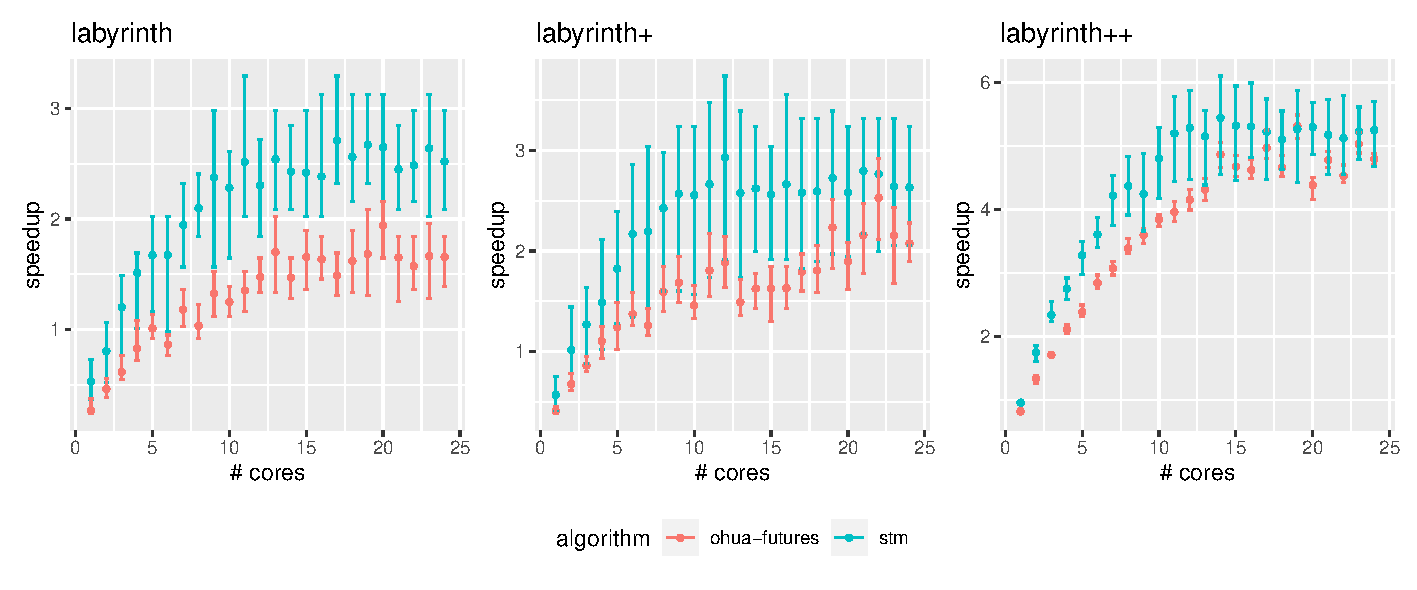
\includegraphics[width=\textwidth,keepaspectratio]{gfx/results/labyrinth_comb}
    \caption{Speedup in the labyrinth application relative to a sequential implementation.}%
    \label{fig:evaluation:labyrinth}
\end{figure}

We already discussed in detail the performance of the \emph{labyrinth} application for Ohua and STM, which is shown in Fig.~\ref{fig:evaluation:labyrinth}, in Chapter~\ref{sec:preliminary}.
Notably, Ohua performs slightly worse than STM, but shows the same overall scaling behavior for more cores while exhibiting less variance in the results.
For labyrinth++, one can not state clearly, which benchmark performs better due to the comparatively large variance in the STM results.
The Software Transactional Memory implementation itself performs just as the original STAMP implementation by Minh et al.~\cite{minh2008stamp}, reinforcing the validity of our implementation.

\begin{figure}
    \centering
    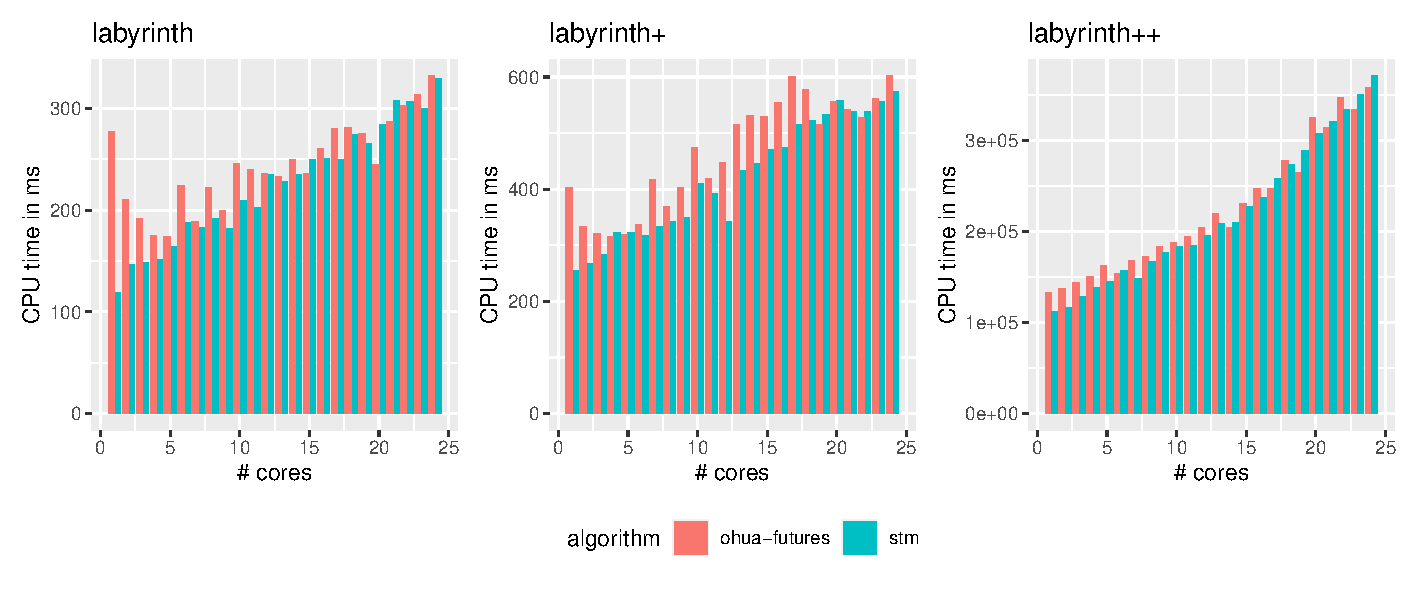
\includegraphics[width=\textwidth,keepaspectratio]{gfx/results/cpu_labyrinth_comb}
    \caption{CPU time used by both frameworks in the labyrinth application.}%
    \label{fig:evaluation:labyrinth-cpu}
\end{figure}

When comparing the CPU time used by both Ohua and STM as shown in Figure~\ref{fig:evaluation:labyrinth-cpu}, we unsurprisingly see an overall growing demand for computation time as creating more threads and moving data between them in itself takes more time.
One can observe the correlation between the time spikes for both applications in the labyrinth+ benchmark and a degraded performance for the respective thread counts.
Due to Ohua's algorithm structure, low thread counts become even less performant for smaller input sets, as fewer threads require more loops of the algorithm, creating a non-negligible runtime overhead.
This becomes irrelevant for larger inputs such as labyrinth++, though.


\begin{figure}
    \centering
    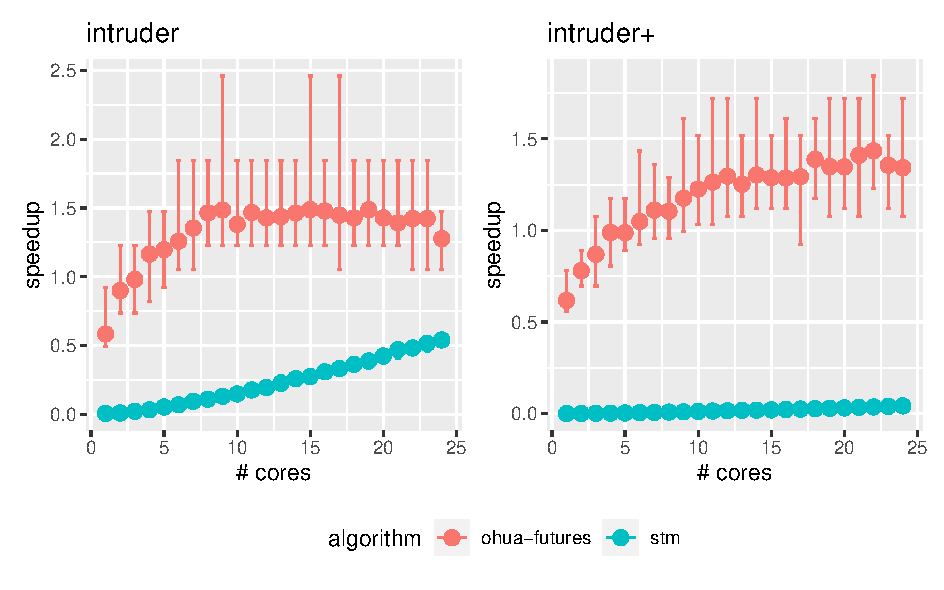
\includegraphics[width=.66\textwidth,keepaspectratio]{gfx/results/intruder_comb}
    \caption{Speedup in the intruder application relative to a sequential implementation.}%
    \label{fig:evaluation:intruder}
\end{figure}

\begin{figure}
    \centering
    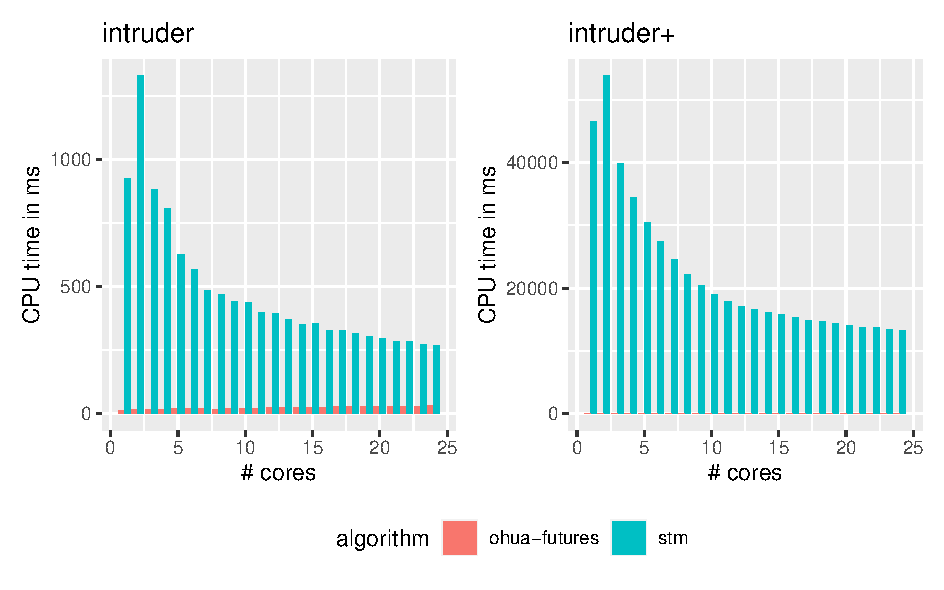
\includegraphics[width=.66\textwidth,keepaspectratio]{gfx/results/cpu_intruder_comb}
    \caption{CPU time used by both frameworks in the intruder application.}%
    \label{fig:evaluation:intruder-cpu}
\end{figure}

For the \emph{intruder} program, both frameworks deliver extremely different results:
STM performance for the small input set (as seen in Fig.~\ref{fig:evaluation:intruder}) is similar to the performance showcased in the reference measurements in Fig.~\ref{fig:evaluation:stamp}, although the curve shape is different, the Rust version showing a slow and steady increase in performance.
The medium sized input set however, produces a rise so flat it almost becomes invisible due to the graph scaling.
We suspect this to be caused by the slow reassembly phase of the benchmark, which operates on a shared HashMap.
Even though we augmented the standard libraries' HashMap implementation with basic transaction handling capabilities like Minh et al.\ did, there is still a lot of contention on these shared data instances, impacting execution times.
This assumption is supported by the immense amount of CPU time used by the STM implementation.
Because of these long execution times for STM we did not attempt measurements for the significantly larger intruder++ input set.

Ohua on the other hand achieves in both cases relatively good speedups of about 1.5 and 1.3 respectively, outperforming Software Transactional Memory.
Particularly interesting is the performance plateau that is reached by Ohua for a medium amount of threads and which is best visible in the smallest input set.
Source of this is the fact that a not insignificant portion of the algorithm runs sequentially in Ohua.
Hence, only a certain speedup may be achieved by parallelizing the application, thus creating a plateau that transitions into declining performance later on when the framework overhead becomes too large.
But as was the case with STM, the intruder+ version performs slightly worse than the smaller input set.
This can be attributed to the increased size of the input set, which takes longer to process during the sequential flow reassembly phase, impairing the speedup achieved by the parallel detection phase.
The aforementioned performance difference is also clearly seen in the use of CPU time which is shown in Figure~\ref{fig:evaluation:intruder-cpu}, where Ohua uses orders of magnitude less CPU time than STM.


\begin{figure}
    \centering
    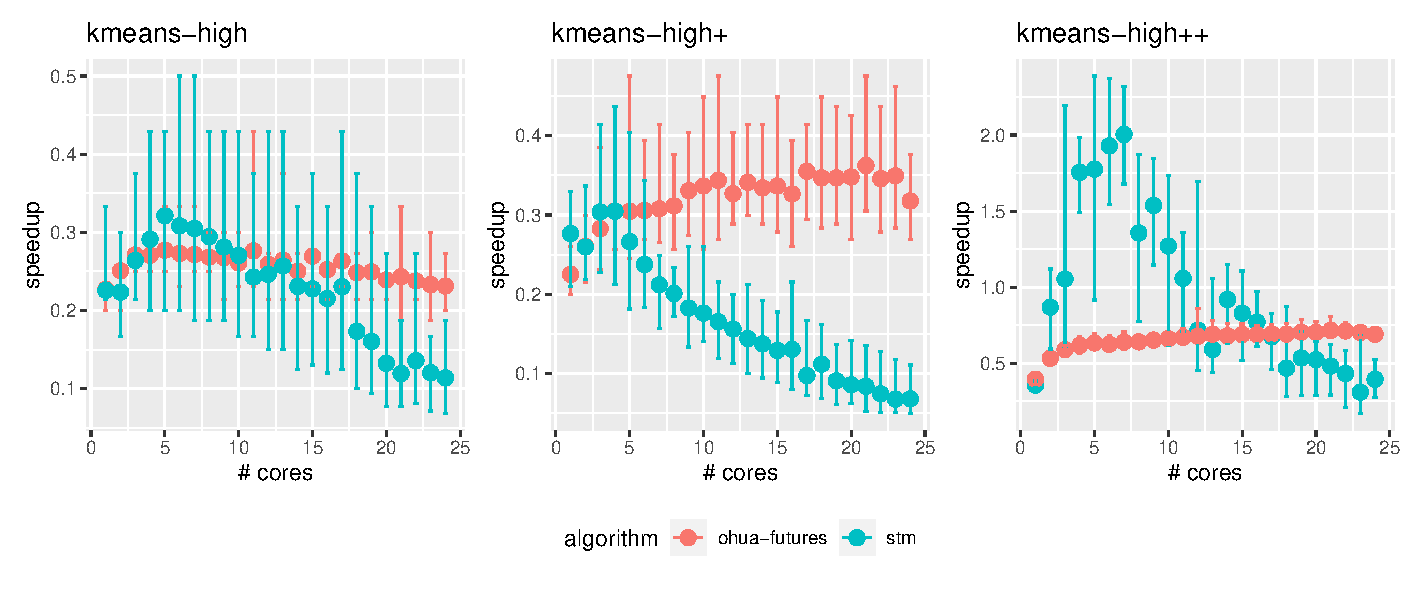
\includegraphics[width=\textwidth,keepaspectratio]{gfx/results/kmeans-high_comb}
    \caption{Speedup in the kmeans-high application relative to a sequential implementation.}%
    \label{fig:evaluation:kmeans-high}
\end{figure}

\begin{figure}
    \centering
    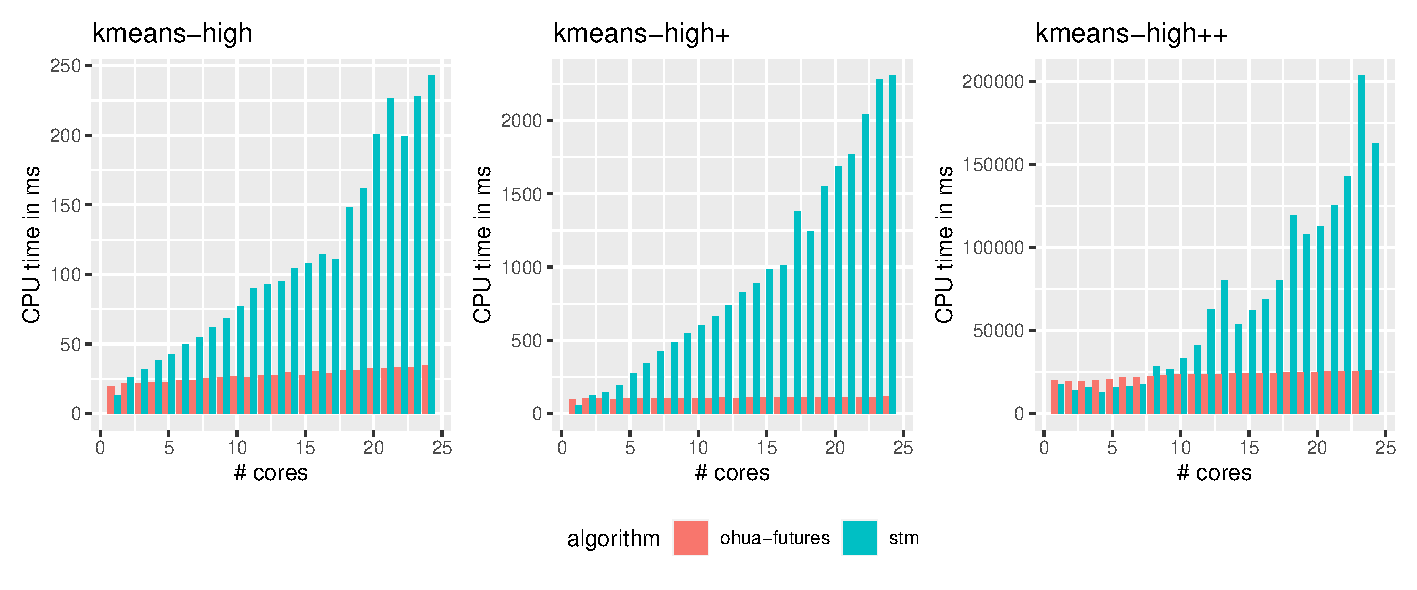
\includegraphics[width=\textwidth,keepaspectratio]{gfx/results/cpu_kmeans-high_comb}
    \caption{CPU time used by both frameworks in the kmeans-high application.}%
    \label{fig:evaluation:kmeans-high-cpu}
\end{figure}

Our \emph{kmeans} results show no clear winner in terms of performance.
Although there were differences in the performance behavior between the high contention and low contention versions of the STAMP benchmark, the STM version written in Rust showcases in Figures~\ref{fig:evaluation:kmeans-high} and~\ref{fig:evaluation:kmeans-low} similar curve shapes for both sets of input data which are completely different from the results in Fig.~\ref{fig:evaluation:stamp}.
This is most likely due to differences in the implementations of both benchmark versions.
C-based programs allow ways of memory sharing that are irreproducible in Rust, forcing us to change some aspects of the program, probably causing these differences.
An example for the differences in what is considered legal memory sharing can be seen in the following snippet of C code:
\begin{minted}{C}
    unsigned long data[] = {1, 2, 3, 4, 5, 6, 7, 8, 9, 10};

    pid_t pid = fork();
    if (pid != 0) {
        int lower = 0;
        int upper = 4;
        // changes elements at indices 0 to 4
        modify_elements(data, lower, upper);
    } else {
        int lower = 5;
        int upper = 9;
        // changes elements at indices 5 to 9
        modify_elements(data, lower, upper);
    }
\end{minted}
There, an array of data (in this example integers, but in \emph{kmeans} it would be observations to classify) is to be manipulated by two concurrent threads.
Since the developer wants to split the work evenly between both threads, she can assign both threads non-overlapping ranges to iterate over and let both threads work directly on the array.
Without any locking, this is risky, as there is no control mechanism ensuring that both threads don't alter the memory regions of the other thread due to a bug in an index calculation or by writing too large portions of data to the array.
Nonetheless, this is the fastest possible implementation (due to the absence of safeguards).
In Rust however, this is impossible.
The language itself does not allow this type of fast yet unsafe memory sharing, as the type system ensures that data shared across threads without locks is read-only.
So, if one wants to implement the same algorithm shown in above listing without locks in Rust, the data must either be copied\footnote{In Rust jargon, this is called a \emph{clone}.} and sent to the respective threads (making a later consolidation of the changes made necessary) or the vector has to be split apart, each part moved into the scope of the respective thread.
Both approaches are time-consuming, as in both cases new memory must be allocated for the new vectors and the data has to be copied or moved, not to mention the time it takes to consolidate the changes made afterwards.

Overall, both benchmark sets show that there is no clear pattern for Ohua's performance with respect to the size of the input set.
Each individual set of input data requires a specific number of iterations before the algorithm converges.
In the Software Transactional Memory version this number is completely unpredictable, fluctuating due to the order in which the elements are processed, as floating point addition offers only a limited precision and is hence not commutative.
Minor differences in the calculation of new centroids therefore can lead to missing the convergence threshold which in turn leads to more computations.
Ohua does this in a fixed amount of iterations as it performs all additions deterministically.
This becomes visible in Ohua's fairly level performance for each input set.
As its determinism guarantees that the computations performed are always in the same order, stripped of any fluctuations caused by non-determinism, speedups and slowdowns mark where the framework either helps to improve performance or where it weighs down execution times.

\begin{figure}
    \centering
    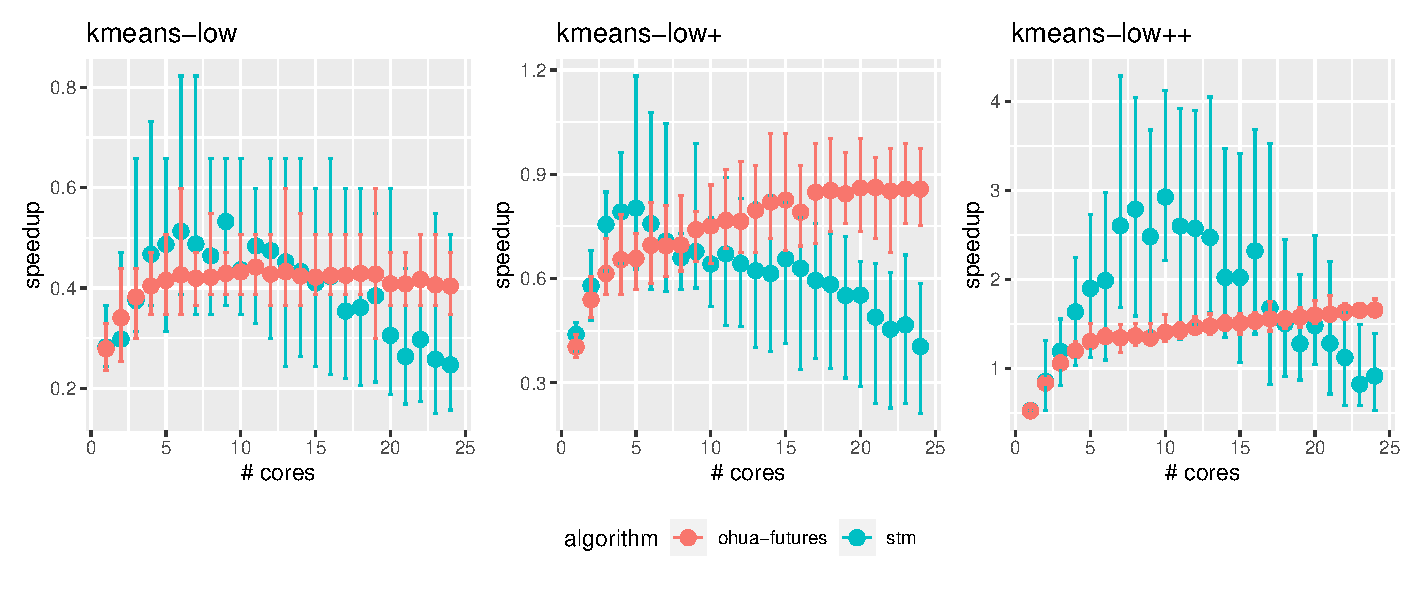
\includegraphics[width=\textwidth,keepaspectratio]{gfx/results/kmeans-low_comb}
    \caption{Speedup in the kmeans-low application relative to a sequential implementation.}%
    \label{fig:evaluation:kmeans-low}
\end{figure}

\begin{figure}
    \centering
    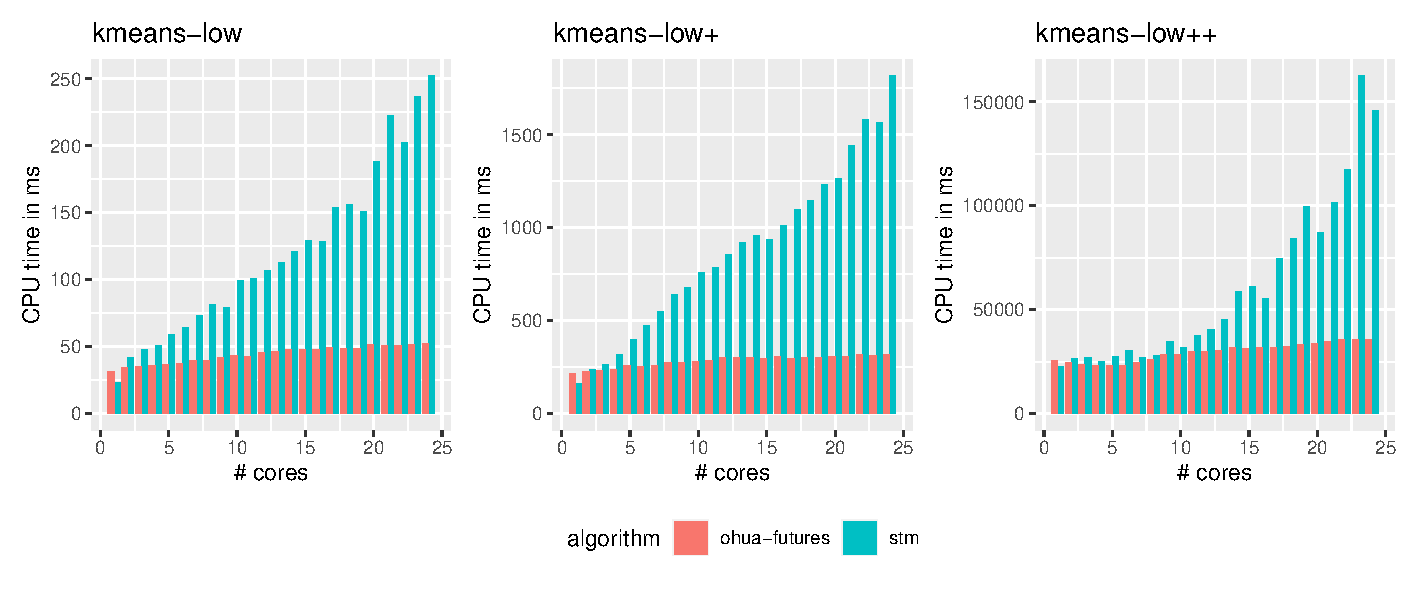
\includegraphics[width=\textwidth,keepaspectratio]{gfx/results/cpu_kmeans-low_comb}
    \caption{CPU time used by both frameworks in the kmeans-low application.}%
    \label{fig:evaluation:kmeans-low-cpu}
\end{figure}

When comparing the utilized CPU times by both frameworks in Figs.~\ref{fig:evaluation:kmeans-high-cpu} and \ref{fig:evaluation:kmeans-low-cpu}, we see that Ohua uses a relatively steady amount of computation time throughout all measurements for kmeans, while STM needs linearly more computation times with increasing thread count.
This can be attributed to an increased number of conflicts due to higher contention, the latter also showing in degrading speedups with increasing thread counts.
All in all, Ohua is on par or outperforms Software Transactional Memory in the smaller two of both kmeans input sets and performs steadily for both large inputs, all while utilizing only a fraction of the CPU time STM needs, meaning it is also using significantly less energy to produce its results.

\begin{figure}
    \centering
    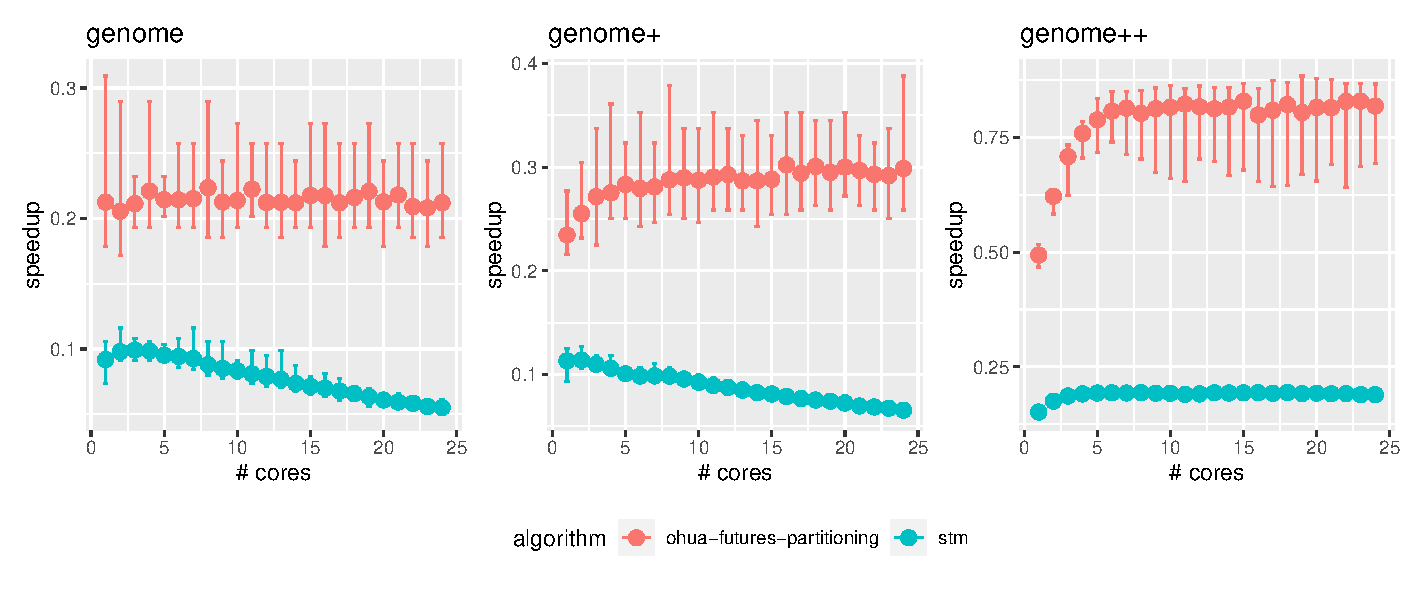
\includegraphics[width=\textwidth,keepaspectratio]{gfx/results/genome_comb}
    \caption{Speedup in the genome application relative to a sequential implementation.}%
    \label{fig:evaluation:genome}
\end{figure}

In \emph{genome}, the curve shapes of our STAMP results from Fig.~\ref{fig:evaluation:stamp} and the results from the STM version in Rust in Fig.~\ref{fig:evaluation:genome} are similar in the way that they exhibit peak performance for a medium amount of threads before it declines.
What's striking is the difference in absolute speedups achieved by our Rust implementation.
Likely causes for this include a by comparison more performant sequential implementation, which is possible as we developed these binaries independently from the other implementations which use one of the two frameworks while Minh et al.\ basically reuse the STM implementation, only removing any TM and threading code from it.
Alternatively, it could be because of higher framework overheads, either within the \texttt{rust-stm} library itself or in our custom STM-ready data structures.
Ohua manages to achieve clearly better speedups in all three test cases.
The execution times remain relatively similar, indicating a steady amount or overhead, although we see an increasing CPU usage in Figure~\ref{fig:evaluation:genome-cpu}, indicating the increasing framework overhead.
But due to the large portions of still sequential code, i.e., the nucleotide sequence deduplication, no real performance gains can be made.

\begin{figure}
    \centering
    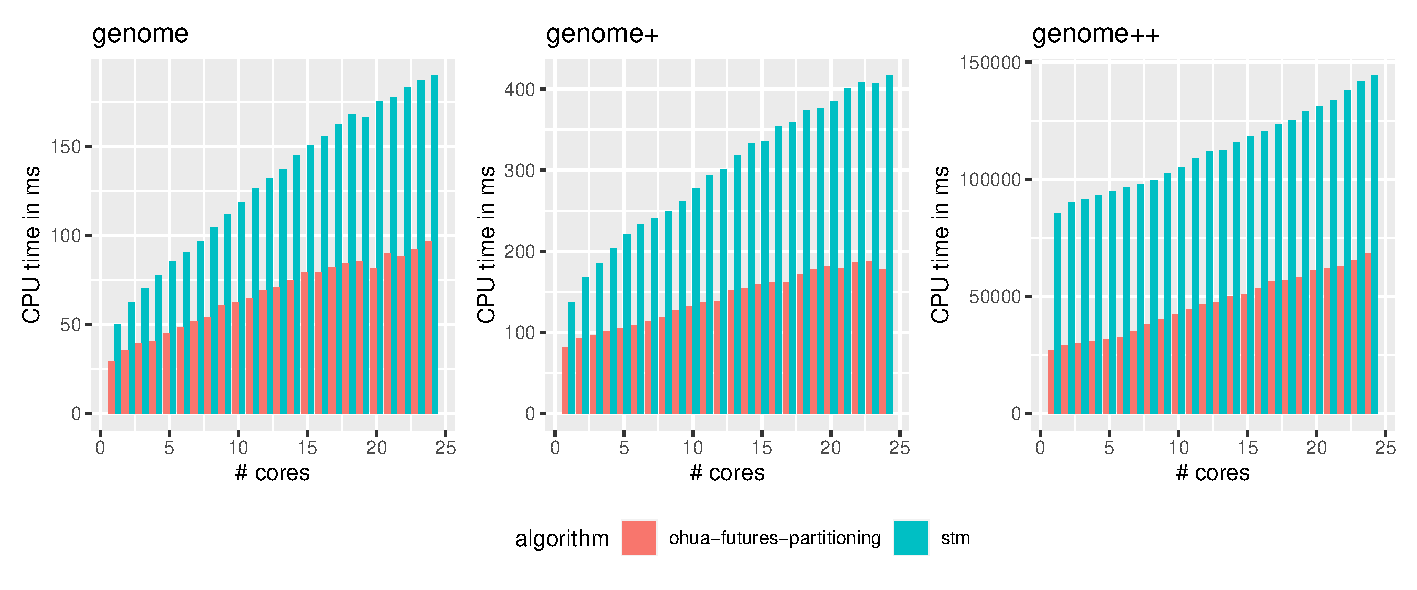
\includegraphics[width=\textwidth,keepaspectratio]{gfx/results/cpu_genome_comb}
    \caption{CPU time used by both frameworks in the genome application.}%
    \label{fig:evaluation:genome-cpu}
\end{figure}


\section{Summary}%
\label{sec:evaluation:summary}

In general, the experiments we've conducted have shown that Ohua's deterministic execution model does indeed lead to less variance in execution times\footnote{This is not immediately visible in the speedup plots in Chapter~\ref{sec:evaluation:benchmarks}, due to the formula used to determine speedup.}.
Our achieved results are on par with those of STM in applications like the labyrinth benchmark, where isolating and exploiting state-free parallelism was relatively easy.\todo{Explain importance of TF2?}
Technically, we also outperformed Software Transactional Memory in the intruder and genome benchmarks but as STM achieved in both cases subpar results, it should be evaluated whether the STM library used can be optimized for a performance comparable to the C-based implementation before judging about this.

With the kmeans and genome benchmarks, it became apparent that not all shared state applications offer the same amount of parallelism exploitable using the transformations we proposed in Chapter~\ref{sec:transformations}.
In fact, it became apparent that of the various forms of irregular applications tested, the one exhibiting amorphous data parallelism could be parallelized best: the labyrinth benchmark.
It is the only one of the four algorithms we implemented that displays the characteristics of amorphous data parallelism we explained in Chapter~\ref{sec:background:irregular:adp}.
This may indicate that Ohua would be most effective when targeting this type of applications in particular, as our batching transformations presented in chapters~\ref{sec:transformations:tf15} and~\ref{sec:transformations:tf2} enable us to handle the state updates found in this type of applications.
To verify this, future work should implement other programs from the STAMP suite that contain amorphous data parallelism such as the \emph{yada} and \emph{ssca2} algorithms.
But even in the non-amorphous cases we tested Ohua on, we saw a significantly lower CPU usage, and by extension power consumption, for Ohua than for STM.
The absence of contention in Ohua's model is the key reason for this conservation of resources.

Overall, Ohua would indeed seem to be a promising replacement for STM-based shared state applications.
While it is clearly not suited to be used for every type of shared state program, so is STM.
Performance-wise Ohua will not always outperform Software Transactional Memory but manages to at least be on par with it, while yielding other positive properties like a deterministic execution model, often better energy efficiency, and easier to work with code bases due to the elimination of parallelism abstractions.

% - present benchmark results -- maybe for the manual Ohua implementation as well, if results differ
% - discuss why we perform better/worse at certain points
% - we see the determinism!
% - discuss energy usage etc

% !TEX root = ../thesis.tex
%
\chapter{Related Work}
\label{sec:related}

Before OHua, various other frameworks for parallel programming hahve been proposed that could serve as a replacement for \emph{Software Transactional Memory} to mitigate some of the shortcomings of the original proposal by Shavit et al.~\cite{shavit1997software}.
This chapter will briefly present some of this related work.

\section{Chocola: Combining multiple concurrency models}
According to Van Roy et al.~\cite{van2004concepts}, most concurrency models can be grouped into three different categories: deterministic, message-passing and shared memory models.
In a study, Swalens et al.~\cite{swalens2018chocola} found that developers often employ multiple concepts from different categories to solve their tasks.
They regard this interleaving of multiple concepts as highly dangerous, as each concurrency model comes with its own set of restrictions on what may or may not be done in the program in order to uphold their individual guarantees.
Mixing two or more models in an application may void some of these guarantees, a fact mose developers are not aware of, as the semantics of this nesting are usually not well-defined.
For example, transactions (a shared-memory model) provide isolation\footnote{Isolation ensures, that one transaction can never see the changes made by another transaction until the latter has comitted. Various levels of isolation have been defined, but Swalens et al.~\cite{swalens2018chocola} were only interested in serializability.} as a guarantee.
However, if futures (a deterministic model) are used inside of transactions, this guarantee is voided, unbeknownst to the developer.

As a solution, and to account for this culture of mixing several concurrency models, the authors propose \emph{Chocola}~\cite{swalens2018chocola}, a unified framework of futures, transactions and actors (a message-passing model).
Chocola is a fork of the Clojure programming language that comes with native support for all three concepts.
Ih their work, Swalens et al. provide well-defined semantics for the combination of two concurrency models.
When defining and implementing their language, they attempted to uphold as much of the original guarantees the individual models offered as possible when combining them, e.g., by altering how futures behave inside a transaction.
For the most part they succeeded, although Determinancy was a guarantee they could often not retain.

To evaluate their work the authors also re-implemented a subset of the STAMP benchmark suite using Chocola.
However, they only tested 4 out of 8 benchmarks, as they argue that only the four selected ones offered any potential for enhancements by combining transactions with another concurrency model.
Swalens et al. reported speedups of 2.3 for a Chocola-based labyrinth implementation, as compared to a speedup of 1.3 for a concentional STM implementation.
Nevertheless, it remains unclear how the authors achieved these measurements, as this is not discussed in their work.
Judging from their references to previous work~\cite{swalens2016transactional, swalens2017transactional}, these speedups may refer to a one-threaded run of the unchanged STM run instead of a sequential implementation.

A significant advantage of this approach is, that it allows the combination of several different concurrency models while offering well-defined and fomralized semantics.
This makes the development of complex software easier for developers as they do not have to put too much thought in the ramifications of this combination.
On the other hand side is this offering of multiple concurrency models also the frameworks' hugest disadvantage.
Developers now don't have to learn how to currectly use one, but three different concepts with different guarantees attached.
Resulting code is so extremely tailored towards the use of these different concepts and their interaction between one another that migrating the code to another framework becomes virtually impossible, depending on how many of Chocola's features are used.
Applications developed with this framework also contain many (potentially different) concurrency abstractions.
In that regard, developing parallel programs might become easier, but understanding and reasoning about them becomes much harder, especially compared to Ohua, which does not expose any abstractions and shields the developer completely from having to reason about concurrency, as this is exploited at compile-time.\todo{Write more comparison?}

\section{Software Lock Elision}
Roy et al.~\cite{roy2009runtime} detail in their work the problems of migrating lock-based code to a Transactional Memory framework.
If done incorrectly, the semantics of the code may change due to the different behavior of transactions compared to locks, leading to different results.
Hence, they propose a Software Lock Elision runtime that builds upon lock-based code and allows threads to speculatively execute lock-based critical sections in parallel.
This framework features an optimistic execution model and detects conflicts between accesses by concurrent threads dynamically.
In this regard, it functions similar to Software Transactional Memory.
But additionally, Software Lock Elision takes a best effort approach on its implementation:
A fallback to acquiring locks without any speculation is possible, e.g., when the speculative state overflows the cache, when using nested locks or when performing an operation that only works non-speculatively (such as waiting for a condition variable).
Roy et al. state that their system is only tailored towards workloads with high contention and a low number of conflicts, as only then using locks becomes a liability.\todo{Or: "too much overhead"?}

\begin{figure}
    \missingfigure[figwidth=7cm]{Adaption of the figure from the original paper}
    \caption{The workflow of the Software Lock Elision runtime. Adapted from Roy et al.~\cite{roy2009runtime}.}%
    \label{fig:related:sle}
\end{figure}

As can be seen in Fig.~\ref{fig:related:sle}, their design features both the automatic and the manual use of SLE.
A developer may either annotate their lock-based code to explicitly use Software Lock Elision at certain points or profile the locks in their binary and apply binary rewriting systems to add a SLE runtime to the application\footnote{In their work, Roy et al. discuss the design for an automated SLE runtime but left an actual implementation to future work. As of today, no follow-up work detailing an actual implementation has been provided.}.
The runtime is designed to retain maximal fairness towards non-speculative locks by prioritizing them over threads holding the same lock speculatively.
The authors also tried to ensure the isolation between speculative and non-speculative work and to add support for application-specific lock types.

To evaluate their work, Roy et al.\ implemented 6 out of 8 STAMP benchmarks\footnote{They reported 2 benchmarks, yada~\& bayes, to not run on their systems anymore.} usin manually-annotated SLE code.
For the kmeans, intruder and ssca2 benchmarks the authors reported speedups significantly higher than those of the original STM implementation.\todo{grafik hier?}
However, the SLE runtime failed to achieve good results for genome, labyrinth and vacation, sometimes only reaching 25-50~\% of the STM speedup.
Interestingly, the framework only achieved good performances in benchmarks with short transactions and at most a medium amount of time spent in transactions, as can be seen in table~\ref{tab:experiments:categorization}.

Overall, this type of automated approach to enhance lock-based code with speculation looks very promising.
It allows the use of STM concepts within lock-based code, which enables developers to easily improve performance of their existing code.
But this requires the use of lock-based code.
The authors make the correct usage of locks a prerequisite in their work, although this is the hardest aspect of lock-based programming, as we discussed in chapter~\ref{sec:background:stm}.
Therefore, an abstraction-free approach to concurrent programming, like Ohua, might be preferrable to avoid having developers write locking code manually.



% !TEX root = ../thesis.tex
%
% \chapter{Future Work}
% \label{sec:future}

% !TEX root = ../thesis.tex
%
% \chapter{Conclusions}
% \label{sec:conclusion}

% --------------------------
% Back matter
% --------------------------
%
{%
\setstretch{1.1}
\renewcommand{\bibfont}{\normalfont\small}
\setlength{\biblabelsep}{0pt}
\setlength{\bibitemsep}{0.5\baselineskip plus 0.5\baselineskip}
\printbibliography[nottype=online]
\newrefcontext[labelprefix={@}]
\printbibliography[heading=subbibliography,title={Web pages},type=online]
}
\cleardoublepage

% TODO: Keep these two things?
\listoffigures
\cleardoublepage

\listoftables
\cleardoublepage

% tmp
\todototoc
\listoftodos
\cleardoublepage

% \lstlistoflistings
% \cleardoublepage

\appendix\cleardoublepage
% \input{content/chapter-appendix}       % INCLUDE: appendix

% \cleardoublepage
% \input{content/colophon}

\cleardoublepage
% !TEX root = ../thesis.tex
%
%************************************************
% Declaration
%************************************************
\pdfbookmark[0]{Declaration}{Declaration}
\chapter*{Declaration}
\label{sec:declaration}
\thispagestyle{empty}

I hereby certify that this thesis has been composed by me and is based on my own work, unless stated otherwise.
No other person's work has been used without due acknowledgement in this thesis.
All references and verbatim extracts have been quoted, and all sources of information, including graphs and data sets, have been specifically acknowledged.
\bigskip

\noindent\textit{\thesisUniversityCity, \thesisDate}

\smallskip

\begin{flushright}
	\begin{minipage}{5cm}
		\rule{\textwidth}{1pt}
		\centering\thesisName
	\end{minipage}
\end{flushright}

%*****************************************
%*****************************************

\clearpage

\newpage
\mbox{}

% **************************************************
% End of Document CONTENT
% **************************************************
\end{document}
